\documentclass[krantz1,a4paper,11pt,ChapterTOCs,twoside,openright]{krantz}
%\usepackage{fixltx2e,fix-cm}   
\usepackage{amssymb}
\usepackage{amsmath}
\usepackage{graphicx}
\usepackage{subfigure}
\usepackage{makeidx}
\usepackage{multicol}
\usepackage[bottom]{footmisc} % places footnotes at page bottom
\usepackage[normalem]{ulem}	  % for strike-through of text with \sout{}
% \usepackage[bottom]{footmisc} % places footnotes at page bottom
% \usepackage[normalem]{ulem}	  % for strike-through of text with \sout{}
\usepackage[numbers,sort&compress]{natbib}

\usepackage{bm}
%\usepackage[labelfont={small,bf},textfont=small]{caption}
%\usepackage{subcaption}
%\usepackage{colortbl}
%\usepackage[margin=10pt,font=small,labelfont=rm,labelsep=endash]{caption}

%\usepackage{hyperref}

\frenchspacing
\tolerance=5000

\makeindex

\newtheorem{theorem}{Theorem}
\newtheorem{exercise}{Exercise}[chapter]
\newtheorem{example}{Example}
\newtheorem{definition}{Definition}
\newtheorem{proof}{Proof}

\newcommand{\hbindex}[1]{\hl{#1}\index{#1}}  %highlights index entries
\def\smallgamma{{\scriptscriptstyle \gamma}}
\def\smallone{{\scriptscriptstyle 1}}
\def\smallE{{\scriptscriptstyle E}}
\def\smallQ{{\scriptscriptstyle Q}}
\def\smallZ{{\scriptscriptstyle Z}}
\def\smallXC{{\scriptscriptstyle XC}}
\def\smallDFT{{\scriptscriptstyle DFT}}
\def\smallGGA{{\scriptscriptstyle GGA}}
\def\smallH{{\scriptscriptstyle H}}
\def\smallKS{{\scriptscriptstyle KS}}
%\def\eqref#1{(\ref{#1})}
\def\angstrom{{\mbox{\AA}}}
\newcommand{\un}[1]{\,\mathrm{#1}}
%\newcommand{\red}[1]{\textcolor{red}{#1}}
\def\rGamma{{\mathrm\Gamma}}
\def\rDelta{{\mathrm\Delta}}
\def\rLambda{{\mathrm\Lambda}}
\def\rOmega{{\mathrm\Omega}}
%%%%%%%%%%%%%%%%%%%%%%%%%%%%%%%%%%%%%%%%%%%%%%%%
% EDITOR COMMANDS
\usepackage[usenames,dvipsnames]{color}
\newcommand{\editor}[2]{%
  \expandafter\newcommand\csname #1note\endcsname[1]{%
    \textcolor{#2}{(\textbf{#1:} ##1)}}%
  \expandafter\newcommand\csname #1\endcsname[1]{%
    \textcolor{#2}{##1}}%
  \expandafter\newcommand\csname #1cancel\endcsname[1]{%
    \textcolor{#2}{\sout{##1}}}%
  \expandafter\newcommand\csname #1change\endcsname[2]{%
    \textcolor{#2}{\sout{##1} ##2}}%
  \newenvironment{#1text}{\color{#2}}{\color{black}}
}
\definecolor{blue}{rgb}{0,0,0.8}
\definecolor{tangerine}{rgb}{0.944,0.522,0}
\definecolor{verde}{rgb}{0,0.6,0}
\editor{LE}{blue}
\editor{SB}{tangerine}

%%%%%%%%%%%%%%%%%%%%%%%%%%%%%%%%%%%%%%%%%%%%%%%%%%%%%%%%%%%%%%%%%%%%%%%%%%
%%%%%%%%%%%%%%%%%%%%%%%%%%%%%%%%%%%%%%%%%%%%%%%%%%%%%%%%%%%%%%%%%%%%%%%%%%
\begin{document}

\frontmatter

\title{THESIS\\
%{\Large(Sottotitolo)}
}
\author{Loris Ercole}

\maketitle

%\cleardoublepage
\thispagestyle{empty}
\vspace*{\stretch{1}}
\begin{flushright}
\Large\itshape
To my parents.
\end{flushright}
\vspace{\stretch{3}}
%\cleardoublepage
%\setcounter{page}{7} %previous pages will be reserved for frontmatter to be added in later.
%\tableofcontents
%\chapter*{Foreword}
I am delighted to introduce the first book on Multimedia Data Mining.  When I came to know about this book project undertaken by two of the most active young researchers in the field, I was pleased that this book is coming in early stage of a field that will need it more than most fields do.  In most emerging research fields, a book can play a significant role in bringing some maturity to the field.  Research fields advance through research papers.  In research papers, however, only a limited perspective could be provided about the field, its application potential, and the techniques required and already developed in the field.  A book gives such a chance.  I liked the idea that there will be a book that will try to unify the field by bringing in disparate topics already available in several papers that are not easy to find and understand.  I was supportive of this book project even before I had seen any material on it.  The project was a brilliant and a bold idea by two active researchers.  Now that I have it on my screen, it appears to be even a better idea.  

Multimedia started gaining recognition in 1990s as a field.  Processing, storage, communication, and capture and display technologies had advanced enough that researchers and technologists started building approaches to combine information in multiple types of signals such as audio, images, video, and  text.  Multimedia computing and communication techniques recognize correlated information in multiple sources as well as insufficiency of information in any individual source.    By properly selecting sources to provide complementary information, such systems aspire, much like human perception system, to create a holistic picture of a situation using only partial information from separate sources.

Data mining is a direct outgrowth of progress in data storage and processing speeds.  When it became possible to store large volume of data and run different statistical computations to explore all possible and even unlikely correlations among data, the field of data mining was born.  Data mining allowed people to hypothesize relationships among data entities and explore support for those.  This field has been put to applications in many diverse domains and keeps getting more applications.  In fact many new fields are direct outgrowth of data mining and it is likely to become a powerful computational tool.\vadjust{\vfill\pagebreak}



%\chapter*{Preface}
Approximately 17 million people in the USA (6{\%} of the
population) and 140 million people worldwide (this number is
expected to rise to almost 300 million by the year 2025) suffer
from \textit{diabetes mellitus}. Currently, there a few dozens of
commercialised devices for detecting blood glucose levels [1].
However, most of them are invasive. The development of a
noninvasive method would considerably improve the quality of life
for diabetic patients, facilitate their compliance for glucose
monitoring, and reduce complications and mortality associated with
this disease. Noninvasive and continuous monitoring of glucose
concentration in blood and tissues is one of the most challenging
and exciting applications of optics in medicine. The major
difficulty in development and clinical application of optical
noninvasive blood glucose sensors is associated with very low
signal produced by glucose molecules. This results in low
sensitivity and specificity of glucose monitoring by optical
methods and needs a lot of efforts to overcome this difficulty.

A wide range of optical technologies have been designed in
attempts to develop robust noninvasive methods for glucose
sensing. The methods include infrared absorption, near-infrared
scattering, Raman, fluorescent, and thermal gradient
spectroscopies, as well as polarimetric, polarization
heterodyning, photonic crystal, optoacoustic, optothermal, and
optical coherence tomography (OCT) techniques [1-31].

For example, the polarimetric quantification of glucose is based
on the phenomenon of optical rotatory dispersion, whereby a chiral
molecule in an aqueous solution rotates the plane of linearly
polarized light passing through the solution. The angle of
rotation depends linearly on the concentration of the chiral
species, the pathlength through the sample, and the molecule
specific rotation. However, polarization sensitive optical
technique makes it difficult to measure \textit{in vivo} glucose
concentration in blood through the skin because of the strong
light scattering which causes light depolarization. For this
reason, the anterior chamber of the eye has been suggested as a
sight well suited for polarimetric measurements, since scattering
in the eye is generally very low compared to that in other
tissues, and a high correlation exists between the glucose in the
blood and in the aqueous humor. The high accuracy of anterior eye
chamber measurements is also due to the low concentration of
optically active aqueous proteins within the aqueous humor.

On the other hand, the concept of noninvasive blood glucose
sensing using the scattering properties of blood and tissues as an
alternative to spectral absorption and polarization methods for
monitoring of physiological glucose concentrations in diabetic
patients has been under intensive discussion for the last decade.
Many of the considered  effects, such as changing of the size,
refractive index, packing, and aggregation of RBC under glucose
variation, are important for glucose monitoring in diabetic
patients. Indeed, at physiological concentrations of glucose,
ranging from 40 to 400 mg/dl, the role of some of the effects may
be modified, and some other effects, such as glucose penetration
inside the RBC and the followed hemoglobin glycation, may be
important [30-32].

Noninvasive determination of glucose was attempted using light
scattering of skin tissue components measured by a
spatially-resolved diffuse reflectance or NIR fre\-quen\-cy-domain
reflectance techniques. Both approaches are based on change in
glucose concentration, which affects the refractive index mismatch
between the interstitial fluid and tissue fibers, and hence
reduces scattering coefficient. A glucose clamp experiment showed
that reduced scattering coefficient measured in the visible range
qualitatively tracked changes in blood glucose concentration for
the volunteer with diabetes studied.




%\listoffigures
%listoftables
%%%\twocolumn
\chapter*{Contributors}

\begin{multicols}{2}
\contributor{Michael Aftosmis}{NASA Ames Research Center}{Moffett Field, California}

\contributor{Pratul K. Agarwal}{Oak Ridge National Laboratory}{Oak Ridge, Tennessee}

\contributor{Sadaf R. Alam}{Oak Ridge National Laboratory}{Oak Ridge, Tennessee}

\contributor{Gabrielle Allen}{Louisiana State University}{Baton Rouge, Louisiana}

\contributor{Martin Sandve Aln{\ae}s}{Simula Research Laboratory and University of Oslo, Norway}{Norway}

\contributor{Steven F. Ashby} {Lawrence Livermore National Laboratory}{Livermore, California}

\contributor{David A. Bader} {Georgia Institute of Technology}{Atlanta, Georgia}

\contributor{Benjamin Bergen} {Los Alamos National Laboratory}{Los Alamos, New Mexico}

\contributor{Jonathan W. Berry} {Sandia National Laboratories}{Albuquerque, New Mexico}

\contributor{Martin Berzins}{University of Utah}{Salt Lake City, Utah}

\contributor{Abhinav Bhatele}{University of Illinois}{Urbana-Champaign, Illinois}

\contributor{Christian Bischof} {RWTH Aachen University}{Germany}

\contributor{Rupak Biswas} {NASA Ames Research Center}{Moffett Field, California}\vspace*{5pt}

\contributor{Eric Bohm} {University of Illinois}{Urbana-Champaign, Illinois}\vspace*{5pt}

\contributor{James Bordner} {University of California, San Diego}{San Diego, California}\vspace*{5pt}

\contributor{George Bosilca} {University of Tennessee}{Knoxville, Tennessee}\vspace*{5pt}

\contributor{Greg L. Bryan} {Columbia University}{New York, New York}\vspace*{5pt}

\contributor{Marian Bubak} {AGH University of Science and Technology}{
Krak{\'o}w, Poland}\vspace*{5pt}

\contributor{Andrew Canning}{Lawrence Berkeley National
Laboratory}{Berkeley, California}

\contributor{Jonathan Carter} {Lawrence Berkeley National
Laboratory}{Berkeley, California}

\contributor{Zizhong Chen} {Jacksonville State University}{Jacksonville,
Alabama}

\contributor{Joseph R. Crobak} {Rutgers, The State University of New
Jersey}{Piscataway, New Jersey}

\contributor{Roxana E. Diaconescu} {Yahoo! Inc.}{Burbank, California}

\contributor{Peter Diener}
{Louisiana State University}{Baton Rouge, Louisiana}

\contributor{Jack J. Dongarra} {University of Tennessee, Knoxville, 
Oak Ridge National Laboratory, and}{University of Manchester}

\contributor{John B. Drake} {Oak Ridge National Laboratory}{Oak Ridge,
Tennessee}

\contributor{Kelvin K. Droegemeier} {University of Oklahoma}{Norman,
Oklahoma}

\contributor{St{\'e}phane Ethier} {Princeton University}{Princeton, New
Jersey}

\contributor{Christoph Freundl}
{Friedrich--Alexander--Universit{\"a}t}{Erlangen, Germany}

\contributor{Karl F{\"u}rlinger} {University of Tennessee}{Knoxville,
Tennessee}

\contributor{Al Geist} {Oak Ridge National Laboratory}{Oak Ridge,
Tennessee}

\contributor{Michael Gerndt} {Technische Universit{\"a}t
M{\"u}nchen}{Munich, Germany}

\contributor{Tom Goodale}
{Louisiana State University}{Baton Rouge, Louisiana}

\contributor{Tobias Gradl}
{Friedrich--Alexander--Universit{\"a}t}{Erlangen, Germany}

\contributor{William D. Gropp} {Argonne National Laboratory}{Argonne,
Illinois}

\contributor{Robert Harkness} {University of California, San
Diego}{San Diego, California}

\contributor{Albert Hartono} {Ohio State University}{Columbus, Ohio}

\contributor{Thomas C. Henderson} {University of Utah}{Salt Lake City,
Utah}

\contributor{Bruce A. Hendrickson} {Sandia National
Laboratories}{Albuquerque, New Mexico}

\contributor{Alfons G. Hoekstra} {University of Amsterdam}{Amsterdam,
The Netherlands}

\contributor{Philip W. Jones} {Los Alamos National Laboratory}{Los
Alamos, New Mexico}

\contributor{Laxmikant Kal{\'e}} {University of
Illinois}{Urbana-Champaign, Illinois}

\contributor{Shoaib Kamil} {Lawrence Berkeley National
Laboratory}{Berkeley, California}

\contributor{Cetin Kiris} {NASA Ames Research Center}{Moffett Field,
California}

\contributor{Uwe K{\"u}ster} {University of Stuttgart}{Stuttgart,
Germany}

\contributor{Julien Langou} {University of Colorado}{Denver, Colorado}

\contributor{Hans Petter Langtangen}
{Simula Research Laboratory and}{University of Oslo, Norway}

\contributor{Michael Lijewski} {Lawrence Berkeley National
Laboratory}{Berkeley, California}

\contributor{Anders Logg}
{Simula Research Laboratory and}{University of Oslo, Norway}

\contributor{Justin Luitjens} {University of Utah}{Salt Lake City, Utah}

\contributor{Kamesh Madduri} {Georgia Institute of Technology}{Atlanta,
Georgia}

\contributor{Kent-Andre Mardal}
{Simula Research Laboratory and}{University of Oslo, Norway}

\contributor{Satoshi Matsuoka} {Tokyo Institute of Technology}{Tokyo,
Japan}

\contributor{John M. May} {Lawrence Livermore National
Laboratory}{Livermore, California}

\contributor{Celso L. Mendes} {University of Illinois}{Urbana-Champaign,
Illinois}

\contributor{Dieter an Mey} {RWTH Aachen University}{Germany}

\contributor{Tetsu Narumi} {Keio University}{Japan}

\contributor{Michael L. Norman} {University of California, San
Diego}{San Diego, California}

\contributor{Boyana Norris} {Argonne National Laboratory}{Argonne,
Illinois}

\contributor{Yousuke Ohno} {Institute of Physical and Chemical Research
(RIKEN)}{Kanagawa, Japan}

\contributor{Leonid Oliker} {Lawrence Berkeley National
Laboratory}{Berkeley, California}

\contributor{Brian O'Shea} {Los Alamos National Laboratory}{Los Alamos,
New Mexico}

\contributor{Christian D. Ott}
{University of Arizona}{Tucson, Arizona}

\contributor{James C. Phillips} {University of
Illinois}{Urbana-Champaign, Illinois}

\contributor{Simon Portegies Zwart} {University of
Amsterdam,}{Amsterdam, The Netherlands}

\contributor{Thomas Radke}
{Albert-Einstein-Institut}{Golm, Germany}

\contributor{Michael Resch} {University of Stuttgart}{Stuttgart,
Germany}

\contributor{Daniel Reynolds} {University of California, San Diego}{San
Diego, California}

\contributor{Ulrich R{\"u}de}
{Friedrich--Alexander--Universit{\"a}t}{Erlangen, Germany}

\contributor{Samuel Sarholz}
{RWTH Aachen University}{Germany}

\contributor{Erik Schnetter}
{Louisiana State University}{Baton Rouge, Louisiana}

\contributor{Klaus Schulten} {University of Illinois}{Urbana-Champaign,
Illinois}

\contributor{Edward Seidel}
{Louisiana State University}{Baton Rouge, Louisiana}

\contributor{John Shalf} {Lawrence Berkeley National
Laboratory}{Berkeley, California}

\contributor{Bo-Wen Shen} {NASA Goddard Space Flight Center}{Greenbelt,
Maryland}

\contributor{Ola Skavhaug}
{Simula Research Laboratory and}{University of Oslo, Norway}

\contributor{Peter M.A. Sloot} {University of Amsterdam}{Amsterdam, The
Netherlands}

\contributor{Erich Strohmaier} {Lawrence Berkeley National
Laboratory}{Berkeley, California}

\contributor{Makoto Taiji} {Institute of Physical and Chemical Research
(RIKEN)}{Kanagawa, Japan}

\contributor{Christian Terboven}
{RWTH Aachen University,}{Germany}

\contributor{Mariana Vertenstein} {National Center for Atmospheric
Research}{Boulder, Colorado}

\contributor{Rick Wagner} {University of California, San Diego}{San
Diego, California}

\contributor{Daniel Weber} {University of Oklahoma}{Norman, Oklahoma}

\contributor{James B. White, III} {Oak Ridge National Laboratory}{Oak
Ridge, Tennessee}

\contributor{Terry Wilmarth} {University of Illinois}{Urbana-Champaign,
Illinois}

\end{multicols}
% \chapter*{Symbols}
\begin{symbollist}{000000}
\symbolentry{$\alpha$}{To solve the generator maintenance scheduling, in the  past, several mathematical techniques have  been applied.}
\symbolentry{$\sigma^2$}{These include integer programming, integer linear programming, dynamic programming, branch and bound etc.}
\symbolentry{$\sum$}{Several heuristic search algorithms have also been developed. In recent years expert systems,}
\symbolentry{$abc$}{fuzzy approaches, simulated annealing and genetic algorithms have also been tested.}
\symbolentry{$\theta\sqrt{abc}$}{This paper presents a survey of the literature}
\symbolentry{$\zeta$}{ over the past fifteen years in the generator}
\symbolentry{$\partial$}{maintenance scheduling. The objective is to}
\symbolentry{sdf}{present a clear picture of the available recent literature}
\symbolentry{ewq}{of the problem, the constraints and the other aspects of}
\symbolentry{bvcn}{the generator maintenance schedule.}
\end{symbollist}

\mainmatter

%\part{Ecosystem-base Impacts of Climate Change}

\chapter{Introduction}  \label{ch:intro}
%\begin{LEtext}
%Struttura del capitolo di intro
%\begin{itemize}
%    \item Intro generale su trasporto termico, importanza nella tecnologia
%    \item difficolta' nel descriverlo, fare modeli: 
%    \item metodi per il calcolo della TC, Green-Kubo method
%    \item ab initio GK - hurdles: gauge invariance, data analysis
%    \item importanza per i vetri, il trasporto termico e' ancora poco capito nei vetri
%    \item esempio: silica glass, importanza della TC, difficolta' coi potenziali classici
%    \item scope of the thesis: tackle these theoretical and practical hurdles, and apply this method to amorphous materials for the first time, to the study of Silica glass
%    \item lista della spesa
%\end{itemize}
%-----
%\end{LEtext}

\vspace{1cm}
\nocite{Ercole2016,Ercole2017,Baroni2018,Bertossa2018}

Heat flow is ubiquitous in nature, it governs a multitude of complex processes, from the evolution of stars and planets to the dynamical stability of biological systems, all the way down to the maintenance of optimal operating conditions in many (nano)technological applications. 
Heat flow determines the internal temperature distribution of out-of-equilibrium systems and the rate of cooling or heating of bodies. 
Therefore the study of thermal transport is fundamental to modeling a multitude of complex systems, and to engineer nanotechnologies, where thermal insulation or dissipation properties have to be properly designed. 
Yet, despite being one the oldest problems of statistical mechanics, a complete theoretical understanding of heat transport is still lacking. 

Transfer of thermal energy occurs via three different mechanisms, that may prevail or coexist in different regimes \cite{Lienhard2017}: \emph{convection}, in which heat is transported by a flow of mass; \emph{radiation}, in which heat is removed from the surface of the hot source by photons; and \emph{conduction}, in which heat transfer is determined by the microscopic dynamics of atoms, or in the case of metals, of conduction electrons. 
In condensed phases and at the molecular scale, conduction is by far the most relevant heat transfer mechanism, and we shall focus on it. 
The first macroscopic theory of heat transport was formulated by Fourier \cite{Fourier1878}, in 1822, who established a proportionality law between the heat current $\mathbf{J}$ and the temperature gradient in the system $\nabla T$:
\begin{equation}
    \mathbf{J} = -\kappa\, \nabla T \,.  \label{eq:Fourier-law}
\end{equation}
The ratio between the heat flux and the temperature gradient defines the \emph{thermal conductivity}, $\kappa$, which is an intrinsic property of the material. 

\medskip

\paragraph{Glass, a quintessential nanotech man-made material}
Although being known and used for more than two thousand years, the last century experienced extraordinary advances in the definition, fabrication, characterisation, and application of glass \cite{Mauro2014}. 
Methods and theory analogous to those employed in the study of crystalline solids have been used to study the electronic, atomic, and micro-structural properties of glass, trying to describe the basic nature of the glassy state, that still represents one of the most difficult open problems in science \cite{MauroFM14}. 
An increased understanding and control of the structure of glass, with both fundamental and fabrication advances, has led to remarkable applications in a variety of fields such as civil engineering, transportation, electronics, photonics, communication, and medicine, many of which are today accepted as the norm. 
Glass is more and more demanded as a high-tech material for consumer electronic devices, and it is going to play a critical role in solving several of the global energy and healthcare challenges of today. 

An atomic-level description of the glassy state is extremely complex due to the lack of long-range order found in crystalline materials, and to the intrinsic non-equilibrium nature of this material. However, thanks to the recent theoretical and experimental advances, glass science is maturing from an empirical discipline to one built upon rigorous scientific principles. 
The glass transition and the processes involved in glass formation are still open questions. 
The chemistry of glasses can be extremely complex: glass compositions are infinitely tunable in chemistry, allowing one to design glasses with tailored mechanical, optical, electrical, magnetic, and thermal properties for specific purposes. 
However this task is far from easy. For example, it was recently discovered that two glasses of identical chemistry may exhibit considerably different short-range structural ordering, thus leading to large differences in the observed properties, a phenomenon called polyamorphism \cite{Huang2004,McMillan2004}. 

In particular, the thermal conductivity is a fundamental property for many industrial and technological applications of glass, ranging from electronics to the insulation efficiency of windows for green architectures, to nuclear waste storage. Despite its importance, ``\emph{thermal conductivity of glass represents largely unexplored territories, ripe for new research efforts}'' (J. Mauro, senior research manager -- Glass Research, Corning Inc.) \cite{MauroFM14}. 
The understanding of thermal conductivity and its structural origin in glasses has been greatly overlooked in the literature and presents several non trivial challenges for atomistic simulations. 
The problem of generating faithful amorphous structures and the correct description of the vibrational properties are the key points that one needs to solve to estimate the thermal conductivity of glasses. 
Moreover, non-periodic systems still lack a theory able to describe the contributions to the thermal conductivity in a way similar to methods widely used for crystalline solids. 



\paragraph{Vitreous silica}
Vitreous silica (a-SiO$_2$, aka fused silica or fused quartz) and silicate glasses in general have been the subject of significant research efforts in the last decades, due to their many technological applications that range from thermal insulation to laser engineering, semiconductor fabrication, and optical communication.
In particular, thanks to its excellent UV transparency, mechanical stability, and chemical durability, silica can be used in many optical applications, such as the diffractive elements and the protective windows of the optics assemblies of inertial confinement fusion facilities. In these facilities, extremely intense nanosecond laser pulses are used and can seriously challenge the durability the optical glasses. It is indeed well established that the small defects or impurities of the glass may cause local lattice heating and melting, resulting in damage craters that will rapidly degrade its optical performance \cite{Miller2004,Canaud2004,Miller2010,Chambonneau2014,Kuzuu1999,Stuart1995,Wong2006,Carr2010,Saito2000}. Moreover, these local damages can be mitigated by using pulsed laser treatments that increase the damage sites to temperatures of $2000-5000\un{K}$ in $10^{-9}$ down to $10^{-12}\un{s}$ and partially restore the desired optical properties \cite{Soules2011}. 
The interpretation of these types of damage processes require the study of thermal properties and the prediction of the thermal conductivity of silica glass, especially in these extreme conditions that experiments cannot probe.

Furthermore, amorphous silica serves as the basis of multicomponent silica glasses, that are adopted for a wide range of special applications. 
To cite an example, borosilicate glasses (BSG) are broadly used to vitrify and immobilize high-level nuclear waste, forming a stable solid matrix that is then stored for very long time \cite{OjovanBook13}. These glasses proved to be one of the most reliable materials to accomplish this task, indeed their intrinsic disorder reduces the effects of radiation damage and their chemical stability and resistance to water corrosion ensures a long and safe storage. A high thermal conductivity favours the efficiency of the fabrication and the stability of the final product, as it entails a faster dissipation of heat generated by radioactive decays. 
Predicting the thermal conductivity of silica also represents the first step towards the prediction of the thermal conductivity of more complicated glasses such as BSG, whose components are characterised by a complex chemistry that is more difficult to model. 

Silica glass has been the subject of many classical MD studies in the last twenty years, that showed that classical force fields can reproduce reasonably well all the structural properties of a-SiO$_2$, but do not describe very well its vibrational spectrum, that instead requires first-principles simulations. 
Its thermal conductivity, that depends on both these properties, still lacks satisfactory and reliable calculations and thus calls for a rigorous study to finally settle the issue. 
Besides, silica also lacks a proper study determining dependence of $\kappa$ on some simulation factors, such as the cooling protocol used to prepare the glass sample and that influences remarkably its structural properties, and the size of system. 


\paragraph{Computing thermal conductivity}
Notwithstanding its fundamental importance, ``\emph{thermal conductivity has proven to be one of the most difficult transport coefficients to calculate}'' \cite{Evans1990} and its simulation is still today a conceptual, no less than practical, challenge to our materials modeling capabilities. 
In order to compute $\kappa$, one needs a microscopic theory that describes the conduction of heat carriers, \emph{i.e.} electrons and lattice vibrations (phonons). Hereafter we will focus only on lattice vibrations, the only carriers contributing to heat transport in \emph{insulators} (the electrons following adiabatically in their ground state), to which we restrict our attention. 
The first microscopic theory of lattice thermal transport was formulated by Peierls, in 1929, and is based on the assumption that phonons obey the Boltzmann transport equation (BTE) \cite{Peierls1929}. 
About thirty years later, Green and Kubo (GK) independently expressed the thermal conductivity, as well as other transport coefficients, by liner response theory in terms of correlation functions of the heat currents \cite{Green1952,Green1954,Kubo1957a,Kubo1957b,Zwanzig1965}:
\begin{equation}
    \kappa \propto \int_{0}^{\infty}\!\langle{J}(t){J}(0)\rangle\, dt, \label{eq:GK-intro}
\end{equation}
where the brackets indicate ensamble averages, thus allowing its computation from simple equilibrium molecular dynamics (MD) simulations. 

In the meantime, a few decades ago, our abilities to understand and predict the properties of materials were boosted by the advent of density functional theory (DFT) \cite{Hohenberg1964,Kohn1965,Martin2008}, which allows computing interactions entirely from quantum mechanics, thus freeing us from the need to leverage prior experimental knowledge, in order to perform MD simulations. 

Recent developments enabled the implementation of the BTE from first principles, thus making it the state of the art technique to compute $\kappa$ of bulk crystalline materials (\emph{e.g.} Si, Ge, diamond \cite{Broido:2007iu,Ward2009}) and nanostructures (\emph{e.g.} graphene and 2D materials \cite{Fugallo2014}). \emph{Ab initio} BTE also provides insights into the mechanisms of heat transport, by breaking down the contributions to $\kappa$ into single carrier properties. 
Nonetheless, the applicability of the BTE approach is limited to periodic materials at low temperatures, where the harmonic approximation of normal modes applies or anharmonic effects are very limited, and it cannot be straightforwardly applied to disordered systems, such as glasses and liquids, were phonons are not even defined, and for which MD is a natural choice. 

On the other hand, MD is set to overcome these limitations: it allows one to study non-periodic and highly anharmonic systems in a straightforward way and to compute their thermal conductivity accounting for full anharmonicity. The only inputs required are the atomic structure and an appropriate interatomic potential, which can be constructed empirically, \emph{e.g.} by fitting previous experimental or \abinitio results using force fields or modern neural networks (classical MD), or directly by first-principles DFT calculations (\abinitio MD, AIMD). 
Once one has these ingredients, $\kappa$ can be computed from equilibrium MD (EMD) or non-equilibrium MD (NEMD) simulations. The latter directly exploits the Fourier law, Eq.~\eqref{eq:Fourier-law}, and applies straightforwardly to finite systems and interfaces, but suffers from severe practical difficulties, such as finite-size and non-linear effects, that have to be carefully accounted for. 
Instead, we focus on EMD simulations, from which the thermal conductivity can be computed directly via the GK equation, Eq.~\eqref{eq:GK-intro}, that only requires an expression for the \emph{heat current}. 
For classical empirical potentials, such expression can be readily obtained as a sum of atomic contributions, containing the atomic coordinates, velocities, and forces. 
On the other hand, a corresponding definition in the framework of DFT was not considered possible until very recently, when it was formulated successfully for the first time \cite{Marcolongo2016}.
Indeed, despite its rigour and simplicity, the GK theory has long been deemed incompatible with DFT, because the total energy cannot be decomposed into individual localized atomic contributions, thus making the heat current ill-defined. 

This conceptual prejudice hindered the development of the GK theory in AIMD simulations for many years. It was only a few years ago that the spurious nature of this belief was recognized through the discovery of a \emph{gauge invariance principle} for transport coefficients \cite{Marcolongo2016,Ercole2016}. 
This principle ensures the value of thermal conductivity ultimately estimated through the GK equation does not depend on the microscopic details that define the energy density, from which the heat current is derived, hence $\kappa$ is well-defined, as any measurable quantity should be. 
However, the problem of univocally defining the atomic energies exists also in classical MD simulations and was recognized in the past, although applications of the GK equation resorted on what was considered the most straightforward definition, without formally justifying this choice. 

On the other hand, despite these important discoveries, experience from classical MD simulations indicates that the practical implementation of the GK theory usually requires very long trajectories to estimate $\kappa$, thus making expensive quantum simulations unfeasible. 
Several expedients have been used in the last twenty years to determine the convergence of the integral in Eq.~\eqref{eq:GK-intro} from trajectories of finite-length, yet it is very surprising that none of these is able to estimate the statistical error of $\kappa$ in an efficient and reliable way. Most of these methods are designed and tested on specific classes of systems, such as crystalline solids (for which, besides, the BTE is the preferable method), but do not work for liquids, disordered or strongly anharmonic systems, or they require extremely long MD simulations. 
We addressed this problem using an innovative data-analysis method based on the \emph{spectral analysis} of stationary time series \cite{Ercole2017}, that provides a rigorous estimation of $\kappa$ with good statistical accuracy from optimally short MD trajectories, for different classes of materials. 
%it is possible to obtain an asymptotically unbiased and consistent estimator for $\kappa$ (\emph{i.e.} the bias and statistical error go to zero in the limit of long simulations). We benchmark it numerically on four different classes of materials and we find that relatively short MD simulations, of the order of one to a few hundreds of picoseconds, are sufficient to obtain a very good statistical error on $\kappa$, of about $\sim 10\%$. 

These two achievements finally demonstrate the feasibility of \abinitio GK simulations of thermal transport and pave the way to their application to previously intractable materials, such as fluids, crystals under extreme conditions, and glasses. 


\medskip

\paragraph{Purpose of this Thesis}
In this thesis we aim to calculate for the first time the thermal conductivity of silica glass at different temperatures, by applying the \abinitio Green-Kubo theory of thermal transport. 
We first show how it is possible to overcome the conceptual and methodological problems mentioned above, that involve the bottom-up definition of a heat current and the estimation of the thermal conductivity from optimally short MD trajectories. 
For this scope, we present the gauge invariance principle for thermal transport coefficients and an innovative data-analysis protocol for transport coefficients. 
We then introduce the problem of simulating an amorphous system with MD, and by means of classical MD simulations we study the effects of sample preparation on the value of thermal conductivity of a-SiO$_2$. 
We use these results as a starting point to run a few first-principles simulations aimed to compute the thermal conductivity of silica at different temperatures using DFT. 

%In the this thesis we present a first application of the \abinitio Green-Kubo theory and the other methodological advances presented. 
%Starting from a classical study, in which we study the effects of many simulation parameters on the thermal conductivity, we then compute $\kappa$ using first-principles simulations at different temperature conditions, and compare the results with experiments. 

\medskip
This thesis is organized as follows. 
Chapter~\ref{ch:green-kubo} introduces the Green-Kubo theory of heat transport. 
Starting from a light review of the theory of hydrodynamic variables and linear response theory, we derive the GK equation for one-component and multi-component systems, and we obtain an expression for the energy current for classical force fields. 
In Chapter~\ref{ch:gauge-invariance} we address the definition of atomic energies and energy densities in interacting systems. We show that there is no unique way to define the heat current, nevertheless the resulting thermal conductivity is well-defined. We prove this statement by numerical simulations and by theory, introducing the principle of gauge invariance of thermal transport coefficients. 
In Chapter~\ref{ch:dft-heat}, after briefly reviewing some of the most recent first-principles simulation techniques of thermal transport, we show how one can derive and compute an \abinitio expression for the energy current in the framework of density functional theory. 
%\LEnote{**discorsi rinormalizzazione**}
Chapter~\ref{ch:data-analysis} is entirely devoted to the practical evaluation of the thermal conductivity from the GK equation. We briefly review all the analysis methods found in the literature, and comment upon their weak points. 
We thus introduce a new technique to evaluate transport coefficients, based on the so-called \emph{cepstral analysis} of time series, and we benchmark it with classical MD simulations for different classes of materials.
In Chapter~\ref{ch:silica} we study the thermal conductivity of a-SiO$_2$ using the \abinitio GK theory. 
We discuss the aspects involved in the atomistic simulation of glass and we simulate silica with classical MD using a popular force field. In particular, we study the dependence of $\kappa$ on the size of the system and the quenching rate used in the virtual vitrification process. 
We then select an optimal system size and simulate one sample with AIMD. 
We compute its thermal conductivity at four different temperatures, and we finally compare the simulation results with experiments. 
Chapter~\ref{ch:conclusions} finally contains our conclusions.

\smallskip
Some parts of Chapter~\ref{ch:green-kubo}, \ref{ch:gauge-invariance}, and \ref{ch:data-analysis} were adapted from the following papers that I have (co-)authored:

\begin{itemize}
    \setlength{\itemsep}{-10pt}
    \item[\textbf{\cite{Ercole2016}}] \printpublication{Ercole2016}. \\
    \item[\textbf{\cite{Ercole2017}}] \printpublication{Ercole2017}. \\
    \item[\textbf{\cite{Baroni2018}}] \printpublication{Baroni2018}. \\
    \item[\textbf{\cite{Bertossa2018}}] \printpublication{Bertossa2018}. \\
\end{itemize}






%\LEnote{**AEROGELS: \small Silica aerogel, a highly porous material first synthesized in the early thirties [1], are currently being produced using a sol–gel process such as hydrolyzing tetramethoxysilane (TMOS) to form silica and methanol, and subsequently dried through supercritical drying together with carbon dioxide [2]. Silica aerogel has several highly desirable properties including being environmentally safe, having high optical transmission as well as large thermal resistance [3]. These properties make silica aerogel very suited for applications such as thermal and acoustic insulation in buildings and appliances, passive solar energy collection devices, and dielectrics for integrated circuits [4]. Also, it is a suitable substitute for chlorofluorocarbon-based plastics in thermal insulation of refrigerators. The most well-known application was in Cherenkov radiators [5] as Cherenkov counters. Another crucial characteristic of aerogels is their extremely low density for a solid, which can go as low as 0.003 g/cm3. Comparatively, the density of air is approximately 0.0012 g/cm3 , which is only three times lower than that of the silica aerogel. This would represent significant weight savings when used in various monolithic structures. **}
  % Introduction
\chapter{Green-Kubo theory of heat transport}  \label{ch:green-kubo}

Our microscopic understanding of heat and mass transport in extended systems is rooted in the Green-Kubo (GK) theory of linear response \cite{Green1954,Kubo1957a}, as applied to the Navier-Stokes equations for the densities of the conserved extensive variables \cite{Kadanoff1963,Forster1975}, which include energy, momentum, and the particle numbers for each molecular species. 
\begin{LEtext}

This work was initiated by Onsager in the thirties \cite{Onsager1931a,Onsager1931b} and carried on by Green and Kubo in the fifties with the theory of linear response \cite{Green1952,Green1954,Kubo1957a,Kubo1957b}. The theory is built on the concept of adiabatic decoupling of the slow long-wavelength components of the densities of conserved extensive quantities (which include energy, momentum, and particle number) \cite{Kadanoff1963}, the so-called \emph{hydrodynamic variables}, from the other atomically fast degrees of freedom. Their work resulted in the celebrated \emph{Green-Kubo equations}, a consequence of the fluctuation-dissipation theorem, that establish a relation between a (non-equilibrium) transport coefficient $\kappa$ and the spontaneous fluctuations of the relevant currents $J$ at equilibrium. Transport coefficients are in fact proportional to their autocorrelation times:
\begin{equation}
\kappa\propto\int_{0}^{\infty}\!\langle{J}(t){J}(0)\rangle\, dt, \label{eq:GK}
\end{equation}
where the brackets indicate ensemble averages over trajectories, and are accessible to equilibrium MD simulations.

In this chapter we briefly walk through the theory that allows the derivation of the Green-Kubo equations for transport coefficients, starting from the definition of the hydrodynamic variables of a system. in Section~\ref{sec:hydrodyn_var}, and the use of linear response theory to connect equilibrium properties to non-equilibrium ones, presented in Section~\ref{sec:linear-response}. In Section~\ref{sec:heat-transport}, we then specialize to the case of heat transport in solids and one component fluids, and the particular case of multi-component fluids, and we derive the expression of the energy flux for systems described by classical force fields.
\end{LEtext}


%%%%%%%%%%%%%%%%%%%%%%%%%%%%%%%%%%%%%%%%%%%%%%%%%%%%%%%%%
\section{Hydrodynamic variables} \label{sec:hydrodyn_var}
The macroscopic processes occurring in condensed matter are often described in terms of \emph{extensive variables}. By definition, the value that such a variable assumes for a system is the sum of the values it has for each of its subsystems. This property allows one to express an extensive variable, $A$, as the integral of a suitably defined density, $a(\mathbf{r})$, as:
\begin{equation}
A[\rOmega]=\int_\rOmega a(\mathbf{r})d\mathbf{r}, \label{eq:A-extensivity}
\end{equation}
where $\rOmega$ is the system volume. Here and in the following boldfaces indicate 3D vectors and Greek subscripts label Cartesian components: $\mathbf{u}= \{u_\alpha\} = \{u_1,u_2,u_3\}$. When an extensive quantity is locally conserved, a current density, $\bm{j}(\mathbf{r},t)$, can be associated to its density in such a way that the two of them satisfy the continuity equation:
\begin{equation}
\frac{\partial a(\mathbf{r},t)}{\partial t} = - \nabla\cdot\bm{j}(\mathbf{r},t), \label{eq:continuity}
\end{equation}
where $\nabla\cdot\bm{j}$ indicates partial differentiation and the middle dot a scalar product (a divergence in this case). In the following the densities and current densities of conserved quantities will be called \emph{conserved densities} and \emph{conserved currents} for short. The space Fourier transform of Eq.~\eqref{eq:continuity} reads:
\begin{equation}
\dot{\tilde a}(\mathbf{q},t) = - i\mathbf{q} \cdot \tilde {\bm{\jmath}} (\mathbf{q},t), \label{eq:kontinuity}\end{equation}
where the overdot indicates a time derivative and the tilde a Fourier transform, so that the longer the wavelength, the slower is the dynamics of a conserved density. We conclude that for long enough wavelengths, conserved densities are adiabatically decoupled from all the other (zillions of) fast atomic degrees of freedom. Note that in this chapter we are using the concept of \emph{adiabatic decoupling} in two distinct senses, depending on the context: to indicate the decoupling of electronic from nuclear degrees of freedom, and that of hydrodynamic variables from fast atomic ones.

The long-wavelength Fourier components of conserved densities are called \emph{hydrodynamic variables}. In macroscopically homogeneous systems, different wavelengths are decoupled from each other, while, as we have seen, the long wavelengths are adiabatically decoupled from all the other degrees of freedom. Let us suppose there are $Q$ conserved extensive variables. In the case of a mono-atomic fluid, for instance, $Q=5$, corresponding to mass (or particle number), energy, and the three components of the momentum. In order to simplify the notation, we set the value of the conserved quantities equal to zero, $A^i=0$, so that their densities, $a^i(\mathbf{r})$, directly refer to the departure from equilibrium, and we indicate by $\bm j^i(\mathbf{r},t)$ the corresponding currents. At equilibrium, all the conserved densities and currents vanish. Off equilibrium, it will be assumed that the wavelength and the time scale of the disturbances are so long that thermal equilibrium still holds \emph{locally}. That is to say, a local temperature, pressure, and chemical potential can be defined, such that, when combined with the densities of extensive variable, they satisfy a local equation of state.

For small enough deviations from equilibrium, the time derivatives of conserved densities are linear combinations of the densities themselves. In the frequency/wavevector domains this condition can be expressed as
\begin{equation}
  -i\omega\tilde a^i(\mathbf{q},\omega) = \sum_j \tilde\rLambda^{ij}(\mathbf{q},\omega) \tilde a^j(\mathbf{q},\omega), \label{eq:Fourier-continuity}
\end{equation}
where the tilde indicates now a space-time Fourier transform: $\tilde a(\mathbf{q},\omega) = \int \mathrm{e}^{-i(\mathbf{q}\cdot \mathbf{r}-\omega t)} a(\mathbf{r},t)d\mathbf{r}dt $. By combining Eq.~\eqref{eq:Fourier-continuity} with the time Fourier transform of Eq.~\eqref{eq:kontinuity}, we obtain the so-called constitutive equations for the (longitudinal components of the) conserved currents:
\begin{equation}
  \tilde{\bm{\jmath}}^i(\mathbf{q},\omega)=i\frac{\mathbf{q}}{q^2} \sum_j\tilde \rLambda^{ij}(\mathbf{q},\omega)\tilde a^j(\mathbf{q},\omega). \label{eq:constitutive-qomega}
\end{equation}
In isotropic media, the $\tilde\rLambda$'s are spherically symmetric functions of $\mathbf{q}$, whereas their value at $\mathbf{q}=0$ vanishes, because a non-vanishing value would imply a non-physical long-range dependence of the currents on density fluctuations, in contrast with our assumption of local thermodynamic equilibrium. The long-wavelength low-frequency limit of the coupling constants can thus be assumed to be $\tilde\rLambda^{ij}(\mathbf{q},\omega) \sim q^2 \lambda^{ij}$, so that the macroscopic ($\mathbf{q}=0$) stationary ($\omega=0$) components of the currents, $\mathbf{J}^i = \frac{1}{\rOmega} \int\bm j^i (\mathbf{r}) d\mathbf{r}$, are related to the corresponding components of the density gradients, $\mathbf{D}^i=\frac{1}{\rOmega}\int\nabla a^i(\mathbf{r})d\mathbf{r}$, through the equations:
\begin{equation}
  \mathbf{J}^i=\sum_j \lambda^{ij}\mathbf{D}^j. \label{eq:constitutive}
\end{equation}
In the following, the macroscopic component of a current will be indicated as a \emph{flux}.

Let $x^i=\frac{\partial S}{\partial A^i}$ be the intensive variable conjugate to $A^i$, where $S$ is the system's entropy, and $\chi^{ij} = \frac{1}{\rOmega} \frac{\partial A^i}{\partial x^j}$ the corresponding susceptibility. For instance, when $A^i$ is the energy of the system, the corresponding conjugate variable is the inverse temperature, $x^i=1/T$, while, when $A^i$ represents the number of particles of a given species, one has $x^i= - \mu^i/T$, $\mu^i$ being the corresponding chemical potential. The hypothesis of local thermodynamic equilibrium allows defining local values of the intensive variables, and we define \emph{thermodynamic forces} as their average gradients: $\mathbf{F}^i= \frac{1}{\rOmega} \int \nabla x^i(\mathbf{r})d\mathbf{r}$. The average density gradients are related to the thermodynamic forces through the susceptibility defined above, as:
\begin{equation}
\mathbf{D}^i=\sum_j\chi^{ij}\mathbf{F}^j .
\end{equation}
By inserting this relation into Eq.~\eqref{eq:constitutive}, one gets:
\begin{equation}
\mathbf{J}^i=\sum_j L^{ij} \mathbf{F}^j, \label{eq:onsager}
\end{equation}
where $L^{ij}=\sum_k\lambda^{ik}\chi^{kj}$. Eq.~\eqref{eq:onsager} expresses the linear relation between fluxes, the $\mathbf{J}$'s, and thermodynamic affinities, the $\mathbf{F}$'s, for which Onsager derived his celebrated reciprocity relations ($L^{ji}=L^{ij}$) from microscopic reversibility \cite{Onsager1931a,Onsager1931b,Casimir1945}. Note that, according to our definition, both the $\mathbf{J}$'s and the $\mathbf{F}$'s in Eq.~\eqref{eq:onsager} do not depend on the size of the system.


%%%%%%%%%%%%%%%%%%%%%%%%%%%%%%%%%%%%%%%%%%%%%%%%
\section{Linear-response theory}  \label{sec:linear-response}
In order to evaluate the $L^{ij}$ phenomenological coefficients appearing in Eq.~\eqref{eq:onsager}, we consider a classical system of $N$ interacting atoms described by the Hamiltonian
\begin{equation}
  H^\circ(\rGamma) = \sum_n\frac{1}{2M_n}(\mathbf{P}_n)^2 + V(\mathbf{R}_1,\mathbf{R}_2,\cdots \mathbf{R}_N), \label{eq:unperturbed_H}
\end{equation}
where $M_n$, $\mathbf{R}_n$, and $\mathbf{P}_n$ are the masses, coordinates, and momenta of the $n$-th particle, $\rGamma=\{\mathbf{R}_n,\mathbf{P}_n\}$ indicates the phase-space coordinates of the entire system, and $V$ is a generic many-body potential. Let us now suppose that the system is subject to an external perturbation that can be described as a linear combination of the conserved densities, $\{a^i(\mathbf{r};\rGamma)\}$, as:
\begin{equation}
   V'(\rGamma,t) = \sum_i \int  v^i(\mathbf{r},t) a^i(\mathbf{r};\rGamma) d\mathbf{r}, \label{eq:perturbation}
\end{equation}
where $a(\mathbf{r};\rGamma)$ is a phase-space function whose ensemble average is the conserved density,
\begin{equation}
    \begin{aligned}
      a(\mathbf{r}) &= \langle a(\mathbf{r};\rGamma) \rangle \\
      & = \int a(\mathbf{r};\rGamma) \mathcal{P}^\circ(\rGamma)d\rGamma,
    \end{aligned}
\end{equation}
$\mathcal{P}^\circ(\rGamma) \propto \mathrm{e}^{-\frac{H^\circ(\rGamma)}{k_BT}}$ is the equilibrium distribution, $k_B$ the Boltzmann constant, and $\{v^i(\mathbf{r},t)\}$ are time-dependent fields that couple to the conserved densities and vanish at $t=-\infty$, when the system is assumed to be in thermal equilibrium at some temperature $T$. Of course, conserved currents are also expected values of some phase-space functions, $\bm{j}(\mathbf{r})=\langle \bm{j}(\mathbf{r};\rGamma)\rangle$. The phase-space functions whose expected values are conserved densities/currents will be referred to as \emph{phase-space samples} of the currents/densities. In the following, when the phase-space dependence of a conserved density/current is explicitly indicated, we will mean a phase-space sample; when it is not a phase-space average will be implied. When a phase-space sample is evaluated along a dynamical trajectory, $\rGamma_t$, the sample function will depend on time and on the initial conditions of the trajectory. Averaging with respect to the initial conditions will result in a time-dependent expected value for the conserved densities (or currents):
\begin{equation}
  \begin{aligned}
    a(\mathbf{r},t) &= \langle a(\mathbf{r};\rGamma'_t)\rangle_0 \\
    &= \int a(\mathbf{r};\rGamma'_t) \mathcal{P}^\circ(\rGamma_0) d\rGamma_0.
  \end{aligned} \label{eq:a(r,t)}
\end{equation}
In Eq.~\eqref{eq:a(r,t)} the notation $\rGamma'_t$ denotes somewhat pedantically that the time evolution in phase space is driven by the perturbed Hamiltonian, $H^\circ+V'$. If it were driven by $H^\circ$, evidently the value of $a$ would be time-independent. In the following, the notation $\rGamma_t$ will indicate an unperturbed time evolution. As an example, the phase-space sample of the particle density can be assumed to be $n(\mathbf{r};\rGamma) = \sum_n \delta (\mathbf{r}-\mathbf{R}_n)$, the corresponding current is $\bm{j} (\mathbf{r}, \rGamma) = \sum_n \delta(\mathbf{r}-\mathbf{R}_n) \mathbf{P}_n / M_n $, and a local external potential is described by: $V'(\rGamma,t)=\sum_n v(\mathbf{R}_n,t)=\int v'(\mathbf{r},t) n(\mathbf{r};\rGamma) d \mathbf{r}$. Note that sample functions are not necessarily univocally defined. Different functions whose phase-space averages coincide in the long-wavelength limit sample the same hydrodynamical variable. More on this in Chapter~\ref{ch:gauge-invariance}.

According to Ref.~\citenum{Green1954}, \citenum{Kubo1957a}, and \citenum{Kubo1957b}, the linear response of the $i$-th conserved current to the perturbation is:
\begin{align}
  j_\alpha^i(\mathbf{r},t) & = \frac{1}{k_B T} \sum_j \int_{-\infty}^t dt' \int d\mathbf{r}' \Bigl \langle j_\alpha^i(\mathbf{r},\rGamma_t)\dot a^j(\mathbf{r}',\rGamma_{t'})\Bigr \rangle_0 v^j(\mathbf{r}',t') \\
  &= \frac{-1}{k_B T} \sum_{j,\beta} \int_{-\infty}^t dt' \int d\mathbf{r}' \Bigl \langle j_\alpha^i(\mathbf{r},\rGamma_t) \partial'_\beta j_\beta^j(\mathbf{r}',\rGamma_{t'})\Bigr \rangle_0 v^j(\mathbf{r}',t') \\
  &= \frac{1}{k_B T} \sum_{j,\beta} \int_{-\infty}^t dt' \int d\mathbf{r}' \left \langle j_\alpha^i(\mathbf{r},\rGamma_{t}) j_\beta^j(\mathbf{r}',\rGamma_{t'})\right \rangle_0 \partial'_\beta v^j(\mathbf{r}',t'). \label{eq:linear-response-c}
\end{align}
The second line follows from the first through the continuity equation, Eq.~\eqref{eq:continuity}, while the third line follows after integrating by parts with respect to $\mathbf{r}'$. The notation $\partial'_\beta=\frac{\partial}{\partial r'_\beta}$ has been used.

By integrating Eq.~\eqref{eq:linear-response-c} all over the space, and assuming space-time homogeneity as well as isotropy, one recovers Eq.~\eqref{eq:onsager} with:
\begin{align}
J^i_\alpha(\rGamma) &= \frac{1}{\rOmega} \int j^i_\alpha(\mathbf{r},\rGamma) d\mathbf{r}, \label{eq:J_def}\\
F^i_\alpha(\rGamma) &= \frac{1}{\rOmega T} \int \partial_\alpha v^i(\mathbf{r},\rGamma) d\mathbf{r}, \label{eq:F_def}\\
L^{ij}_{\alpha\beta} &= \frac{\rOmega}{k_B} \int_0^\infty \left\langle J^i_\alpha(\rGamma_t) J^j_\beta(\rGamma_0)\right\rangle_0 dt. \label{eq:L_def}
\end{align}
This completes the derivation of the Green-Kubo formula for transport coefficients, Eq.~\eqref{eq:GK}, from classical linear-response theory. Onsager's reciprocity relations, $L^{ij}=L^{ji}$ \cite{Onsager1931a,Onsager1931b}, follow from Eq.~\eqref{eq:L_def} leveraging time-translational invariance, $\langle J^i_\alpha(\rGamma_t) J^j_\beta(\rGamma_0) \rangle = \langle J^i_\alpha(\rGamma_0) J^j_\beta(\rGamma_{-t}) \rangle$, and micro-reversibility, $\langle J^i_\alpha(\rGamma_t) J^j_\beta(\rGamma_0) \rangle = \langle J^i_\alpha(\rGamma_{-t}) J^j_\beta(\rGamma_0) \rangle$.


\subsection{Einstein-Helfand expression for transport coefficients and the Wiener-Khintchine theorem}  \label{sec:Einstein}
The celebrated Einstein's relation between the mean-square displacement of a diffusing particle and its velocity auto-correlation function is easily generalized to an arbitrary stochastic process and has in fact been utilized by \citet{Helfand1960} to provide an ``Einstein-like'' expression for transport coefficients.

Let $X_t$ be a stationary stochastic process. One has:
\begin{equation}
  \frac{1}{\mathcal{T}} \left\langle \left| \int_0^\mathcal{T} X_t dt \right|^2 \right\rangle = 2 \int_0^\mathcal{T} \left\langle X_t X_0 \right\rangle dt -\frac{2}{\mathcal{T}} \int_0^\mathcal{T} \left\langle X_t X_0 \right\rangle t \,dt. \label{eq:Einstein-Helfand}
\end{equation}
In the large-$\mathcal{T}$ limit, the second term on the right-hand side of Eq.~\eqref{eq:Einstein-Helfand} can be neglected. 

When the stochastic process is the velocity of a Brownian particle, Eq.~\eqref{eq:Einstein-Helfand} allows one to establish a relation between the diffusion constant of the particle, temperature, and the auto-correlation time of the velocity.  When $X_t$ is the heat flux of a macroscopic body, Eq.~\eqref{eq:Einstein-Helfand} allows one to estimate the thermal conductivity, as given by Eq.~\eqref{eq:GK}, from the asymptotic behavior of the ``energy displacement'' $\mathbfcal{D}(\tau) = \int_0^\tau \mathbf{J}(\rGamma_t) dt $. 
From Eq.~\eqref{eq:L_def} we have that
\begin{align}
    L_{\alpha\beta}^{ij} &= \lim_{\mathcal{T\rightarrow\infty}} \frac{\rOmega}{k_B} \int_0^{\mathcal{T}} \left\langle J^i_\alpha(\rGamma_t) J^j_\beta(\rGamma_0)\right\rangle_0 \left(1 - \frac{t}{\mathcal{T}}\right) dt \nonumber\\
    &= \lim_{\mathcal{T\rightarrow\infty}} \frac{\rOmega}{2k_B\mathcal{T}} \left\langle \int_0^\mathcal{T} J_\alpha^i(\rGamma_t) \int_0^\mathcal{T} J_\beta^j(\rGamma_t) dt \right\rangle_0 .  \label{eq:Einstein-Helfand-Lij}
\end{align}

\paragraph{Power Spctrum}
Eq.~\eqref{eq:Einstein-Helfand} can be easily generalized to the finite-frequency regime, to get:
\begin{equation}
  \begin{aligned}
    S_\mathcal{T}(\omega) &= \frac{1}{\mathcal{T}} \left \langle \left | \int_0^\mathcal{T} X_t \mathrm{e}^{i\omega t}dt \right |^2 \right \rangle \\
    &= 2\mathfrak{Re} \int_0^\mathcal{T} \left \langle X_t X_0 \right \rangle \mathrm{e}^{i\omega t}dt + \mathcal{O}(\mathcal{T}^{-1}).
  \end{aligned}
  \label{eq:Wiener-Khintchine}
\end{equation}
This equation expresses the Wiener-Khintchine theorem \cite{Wiener1930,Khintchine1934}, which states that the expectation of the squared modulus of the Fourier transform of a stationary process is the Fourier transform of its time correlation function, which is usually referred to as the process \emph{power spectral density},
\begin{equation}
  S(\omega) = \int_{-\infty}^\infty \langle X_t X_0 \rangle \,\mathrm{e}^{i\omega t} dt, \label{eq:S(omega)}
\end{equation}
aka the \emph{power spectrum}. In the following the suffix $\mathcal{T}$ will be neglected for simplicity and its value assumed to be sufficiently large as to be considered infinite. More generally, when several conserved currents interact with each other, one can define the \emph{cross-spectrum} of the conserved fluxes as the Fourier transform of the cross time-correlation functions:
\begin{equation}
  \begin{aligned}
    S^{kl}(\omega) &= \int_{-\infty}^\infty \langle X^k_t X^l_0 \rangle \,\mathrm{e}^{i\omega t} dt \\
    &= \frac{1}{\mathcal{T}} \mathfrak{Re} \left\langle \int_0^\mathcal{T} X^k_t \mathrm{e}^{-i\omega t}dt \times \int_0^\mathcal{T} X^l_t \mathrm{e}^{i\omega t}dt \right\rangle + \mathcal{O}(\mathcal{T}^{-1}).
  \end{aligned} \label{eq:Sij(omega)}
\end{equation}
Eqs.~\eqref{eq:Einstein-Helfand} and \eqref{eq:Wiener-Khintchine} indicate that the transport coefficients we are after essentially are the zero-frequency value of the (cross-) power spectrum of the corresponding current(s), a fact that will be instrumental in our approach to data analysis, as explained in Chapter~\ref{ch:data-analysis}. Therefore, Eq.~\eqref{eq:L_def} can be cast into the form:
\begin{equation}
    L^{kl} =\frac{\rOmega}{2 k_B} S^{kl}(\omega=0), \label{eq:GK-S0}
\end{equation}
where the Cartesian indices have been omitted for clarity.


%%%%%%%%%%%%%%%%%%%%%%%%%%%%%%%%%%%%%%%%%%%%%%%%5
\section{Heat transport}  \label{sec:heat-transport}
The above treatment allows one to compute the linear response of a system at thermal equilibrium to a generic mechanical perturbation. Heat transport is determined by temperature gradients that cannot be described by any mechanical perturbation. The concept of temperature distribution implies that the system is locally at thermal equilibrium over lengths and times large with respect to atomic distances and relaxation times. Temperature affects the physical properties of a system through the Boltzmann distribution function. When the temperature is not constant, $T(\mathbf{r})=T+\rDelta T(\mathbf{r})$ ($|\rDelta T| \ll T$), the effects of this inhomogeneity can be formally described by the distribution function:
\begin{align}
  \mathcal{P}(\rGamma) & \propto
  \exp\left[ -\int \frac{e(\mathbf{r};\rGamma)}{k_BT(\mathbf{r})}d\mathbf{r} \right] \\
  &= \exp\left[ -\frac{H^\circ(\rGamma)+V'(\rGamma)}{k_BT} \right],
\end{align}
where $e(\mathbf{r};\rGamma)$ is an energy (Hamiltonian) density, such that $\int e(\mathbf{r};\rGamma) d\mathbf{r} = H^\circ(\rGamma)$. Eq.~\eqref{eq:perturbation} becomes:
\begin{equation}
   V'(\rGamma)=-\frac{1}{T}\int\rDelta T(\mathbf{r})e(\mathbf{r};\rGamma) d\mathbf{r} + \mathcal{O}(\rDelta T^2) . \label{eq:mechanical-perturbation}
\end{equation}
Eq.~\eqref{eq:mechanical-perturbation} shows that the effects of temperature inhomogeneities can be mimicked by a mechanical perturbation coupled to the temperature distribution. From Eqs.~\eqref{eq:onsager} and (\ref{eq:J_def}-\ref{eq:L_def}) we conclude that in a system where the only non-trivial conserved quantity is the energy, the heat (energy) flow is coupled to temperature gradients through the constitutive equation:
\begin{equation}
  \mathbf{J}^\smallE = - \kappa \nabla T, \label{eq:thermal-constitutive}
\end{equation}
where the thermal conductivity $\kappa_{\alpha\beta}= L^{\scriptscriptstyle EE}_{\alpha \beta} / T^2$ (see Eq.~\eqref{eq:onsager}) can be expressed by a Green-Kubo relation in terms of the fluctuations of the energy flux as:
\begin{equation}
  \boxed{ \kappa_{\alpha\beta} =\frac{\rOmega}{k_B T^2} \int_0^\infty \left \langle J^\smallE_\alpha(\rGamma_t) J^\smallE_\beta(\rGamma_0) \right \rangle_0 dt } \label{eq:GK-complete}
\end{equation}
and
\begin{equation}
  \mathbf{J}^\smallE(\rGamma)  = \frac{1}{\rOmega} \int \bm{j}^\smallE(\mathbf{r};\rGamma) d\mathbf{r}. \label{eq:avg-current-density}
\end{equation}
In order to obtain an explicit expression for the energy flux from a microscopic expression for the energy density, we multiply the continuity equation, Eq.~\eqref{eq:continuity}, by $\mathbf{r}$ and integrate by parts, to obtain:
\begin{align}
  \mathbf{J}^\smallE(\rGamma) &= \frac{1}{\rOmega} \int  \dot e(\mathbf{r};\rGamma_t) \,\mathbf{r}\, d\mathbf{r} \label{eq:JE=rdote} \\
  & = \frac{1}{\rOmega} \int
  \left[ \sum_n \left(
    \frac{\partial e(\mathbf{r};\rGamma_t)}{\partial \mathbf{R}_n} \cdot \mathbf{V}_n +
    \frac{\partial e(\mathbf{r};\rGamma_t)}{\partial \mathbf{P}_n} \cdot \mathbf{F}_n
  \right)  \right] \mathbf{r}\, d\mathbf{r}, \label{eq:JE}
\end{align}
where $ \mathbf{F}_n $ is the force acting on the $n$-th atom, and $\mathbf{V}_n=\frac{\mathbf{P}_n}{M_n}$ its velocity.

The manipulations leading from the continuity equation, Eq.~\eqref{eq:continuity}, to Eq.~\eqref{eq:JE} deserve some further comments, as they imply neglecting a boundary term, $\mathbf{J}_{\partial \rOmega} =
\frac{1}{\rOmega} \int_{\partial\rOmega}
 \left( \bm{j}(\mathbf{r}) \cdot \hat{\mathbf{n}} \right)
\mathbf{r} \,d\mathbf{r} $  (where $ \partial\rOmega $ is the boundary of the integration volume and $\hat{\mathbf{n}}$ the normal to it), which in general does not vanish in the thermodynamic limit and is ill-defined in periodic boundary conditions (PBC), as it depends on the definition and choice of the unit cell. The correct way of addressing this problem is to work with the Taylor expansion of the space Fourier transform of the continuity equation, Eq.~\eqref{eq:kontinuity}, and to perform the thermodynamic limit at finite wavelength. The leading non-vanishing term in the Taylor expansion yields Eq.~\eqref{eq:JE=rdote} without any boundary term in the way.


\subsection{Energy flux from classical force fields}
When atoms interact through a classical force field, $V(\mathbf{R}_1,\mathbf{R}_2,\cdots \mathbf{R}_N)$, an energy density can be defined in terms of local atomic energies as:
\begin{align}
  e(\mathbf{r},\rGamma) &= \sum_n \delta(\mathbf{r}-\mathbf{R}_n) e_n(\rGamma), \label{eq:epsilon-classical} \\
  e_n(\rGamma) &= \frac{(\mathbf{P}_n)^2}{2M_n} + v_n(\{\mathbf{R}\}), \label{eq:atomic-energies}
\end{align}
where the $v_n$'s are a set of atomic potential energies whose sum is the total potential energy of the system, $\sum_n v_n=V$, with a short-range dependence on the coordinates of the other atoms. In the presence of long-range forces, this condition is effectively guaranteed by local charge neutrality, which we will assume throughout.
By inserting Eq.~\eqref{eq:epsilon-classical} into Eq.~\eqref{eq:JE}, the energy flux can be cast into the form:
\begin{equation}
  \mathbf{J}^\smallE(\rGamma) =
        \frac{1}{\rOmega} \left[ \sum_n \mathbf{V}_n e_n + \sum_n \mathbf{R}_n
        \left( \mathbf{F}_n \cdot \mathbf{V}_n  + \sum_m \mathbf{V}_m \cdot {\frac{\partial v_n}{\partial \mathbf{R}_m}} \right) \right] \label{eq:J-classical}
\end{equation}

\begin{LEtext}
\paragraph{Two-body poentials}
When the interaction among atoms can be expressed in terms of two-body potentials, one has: $v_m=\frac{1}{2}\sum_n v(\mathbf{R}_n- \mathbf{R}_m)$ and $\mathbf{F}_{n m} = - \frac{1}{2} \nabla_{\mathbf{R}_n} v(\mathbf{R}_n- \mathbf{R}_m)$, where $\mathbf{F}_{n m} = - \frac{\partial v_m}{\partial \mathbf{R}_n}$ is the contribution of the $m$-th atom to the force acting on the $n$-th atom, $\sum_m \mathbf{F}_{n m} = \mathbf{F}_{n}$, and $\mathbf{F}_{n m} = -\mathbf{F}_{m n}$. 
Here we implicitly assumed that the interaction energy is equally partitioned between atoms $m$ and $n$. In Chapter~\ref{ch:gauge-invariance} we shall see this is not the only possible choice, with far-reaching consequences on the theory of heat transport.
The energy flux becomes:
\begin{equation}
    \mathbf{J}^\smallE(\rGamma) =
       \frac{1}{\rOmega} \left[ \sum_n \mathbf{V}_n e_n + \sum_{n,m} (\mathbf{R}_n-\mathbf{R}_m) \mathbf{F}_{n m} \cdot \mathbf{V}_n \right]. \label{eq:J-classical-2body}
\end{equation}
Notice that this expression is also well-defined in PBC.

\begin{figure}[tb]
    \centering
    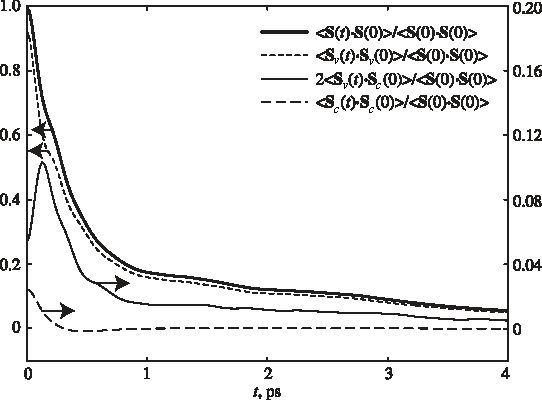
\includegraphics[width=8cm]{chapters/chapter2/figures/McGaughey-argon-contributions.pdf}
    \caption{Breakdown of the energy flux autocorrelation function $\langle\mathbf{J}^\smallE(t)\cdot\mathbf{J}^\smallE(t)\rangle$ of LJ fcc solid argon at $50\un{K}$ into the three terms of Eq.~\eqref{eq:JtJ0-components}. Note that the total ACF and the virial component correspond to the left vertical axis, while the cross and convection curves correspond to the right axis. Reproduced from Ref.~\cite{McGaughey2006}.}
    \label{fig:argon-convective}
\end{figure}

The first term on the right-hand side of Eq.~\eqref{eq:J-classical},
\begin{equation}
    \mathbf{J}^\smallE_c = \frac{1}{\rOmega} \sum_n \mathbf{V}_n e_n , \label{eq:J-convective}
\end{equation}
is often called \emph{convective} (or \emph{kinetic}) and the second term,
\begin{equation}
    \mathbf{J}^\smallE_v = \frac{1}{\rOmega} \left[ \sum_{n,m} (\mathbf{R}_n-\mathbf{R}_m) \mathbf{F}_{n m} \cdot \mathbf{V}_n \right], \label{eq:J-virial}
\end{equation}
is often called \emph{virial} (or \emph{potential}).
\citet{Fan2015} and \citet{Carbogno:2017gc}, for example, adopt this nomenclature and state that the convective term $\mathbf{J}^\smallE_c$ ``\emph{gives no contributions to the conductivity tensor in solids, as mass transport is negligible}''.
We feel that the wording ``convective'' is somewhat misleading in this context, as the contribution of the convective current $\mathbf{J}^\smallE_c$ to the heat conductivity may not vanish even in the absence of convection, especially in softer solid materials. 
Using Eqs.~\eqref{eq:J-convective} and \eqref{eq:J-virial}, the energy flux autocorrelation function can be split into 3 terms:
\begin{equation}
    \langle\mathbf{J}^\smallE(t)\cdot\mathbf{J}^\smallE(t)\rangle = \langle\mathbf{J}_c^\smallE(t)\cdot\mathbf{J}_c^\smallE(t)\rangle + 
    2\langle\mathbf{J}_c^\smallE(t)\cdot\mathbf{J}_v^\smallE(t)\rangle + 
    \langle\mathbf{J}_v^\smallE(t)\cdot\mathbf{J}_v^\smallE(t)\rangle . \label{eq:JtJ0-components}
\end{equation}
Their contributions to thermal conductivity were computed by \citet{McGaughey2006} for a LJ fcc argon crystal at $50\un{K}$ (the breakdown of $\langle\mathbf{J}^\smallE(t)\cdot\mathbf{J}^\smallE(t)\rangle$ into the three terms of Eq.~\eqref{eq:JtJ0-components} is shown in Fig.~\ref{fig:argon-convective}). They found that while the convection contribution $\langle\mathbf{J}_c^\smallE(t)\cdot\mathbf{J}_c^\smallE(t)\rangle$ was indeed small ($\sim 1\%$), the contribution of the cross term $2\langle\mathbf{J}_c^\smallE(t)\cdot\mathbf{J}_v^\smallE(t)\rangle$ is not insignificant ($\sim 10\%$). 
The relative contributions of the convective and cross terms increase as the temperature goes up and anharmonic effects inhibit ``pure'' conduction. 
The absolute values of the convective contribution remains the same with increasing temperature, whereas the virial and cross term contributions decrease. \LEnote{<-- check this**}
While the convective term may not be as important for materials with higher thermal conductivity, in general, its contribution and that of the cross term should be checked before assuming they are negligible. Some further comments on this issue in Sec.~\ref{sec:carbogno}. 

In the literature the nomenclature is often confusing, and the relative contributions of each term is often not very well known. 
For example, \citet{Vogelsang1987} divide the energy currents in two terms \cite{McQuarrie2000}: a ``\emph{kinetic}'' part, defined as
\begin{equation}
    {\mathbf{J}^\smallE_k}' = \frac{1}{\rOmega} \frac{(\mathbf{P}_n)^2}{2M_n} \mathbf{V}_n ,
\end{equation}
and a ``\emph{potential}'' part, defined as
\begin{equation}
    {\mathbf{J}^\smallE_p}' = \frac{1}{\rOmega} \left[ \sum_n  v_n(\{\mathbf{R}\}) \mathbf{V}_n + \sum_{n,m} (\mathbf{R}_n-\mathbf{R}_m) \mathbf{F}_{n m} \cdot \mathbf{V}_n \right] .
\end{equation}
They find that ${\mathbf{J}^\smallE_k}'$ is negligible in solids, where atomic diffusion does not occur.
\citet{Kinaci2012}, instead, use the Einstein formulation and define a ``\emph{kinetic}'' term
\begin{equation}
    {\mathbf{J}^\smallE_k}'' = \frac{1}{\rOmega} \left[ \frac{(\mathbf{P}_n)^2}{2M_n} \mathbf{V}_n + \sum_{n,m} (\mathbf{R}_n-\mathbf{R}_m) \mathbf{F}_{n m} \cdot \mathbf{V}_n \right],
\end{equation}
and a ``\emph{potential}'' term
\begin{equation}
    {\mathbf{J}^\smallE_p}'' = \frac{1}{\rOmega} \sum_n  v_n(\{\mathbf{R}\}) \mathbf{V}_n ,
\end{equation}
and conclude that in perfect solid systems, where diffusion is highly improbable, ${\mathbf{J}^\smallE_p}''$ contribution to thermal conductivity is negligible.

Finally, an alternative definition of the heat current can be used when dealing with solids \cite{Ladd1986}:
\begin{equation}
    \mathbf{J}^\smallE(\rGamma) =
       \frac{1}{\rOmega} \sum_{n,m} (\mathbf{R}_n^0 -\mathbf{R}_m^0) \mathbf{F}_{n m} \cdot \mathbf{V}_n , \label{eq:J-leyla}
\end{equation}
where $\mathbf{R}_n^0$ denotes the average atomic position of atom $n$. One should not confuse this expression with neglecting the convection part of the heat current. For a solid, Eq.~\eqref{eq:J-leyla} will give the same thermal conductivity as Eq.~\eqref{eq:J-classical-2body}, as demonstrated in Sec.~\ref{sec:carbogno}.


\paragraph{Many-body potentials}
In the case of a many-body potential interaction, if the atomic potential energy can be written as a function of the distance vectors $\mathbf{R}_{nm}=\mathbf{R}_n-\mathbf{R}_m$, as $v_n = v_n(\mathbf{R}_{1n},\mathbf{R}_{2n},\cdots,\mathbf{R}_{Nn})$, the force acting on atom $n$ can be written as \cite{Fan2015,Hardy2016}:
\begin{align}
    \mathbf{F}_n &= -\sum_m \frac{\partial v_m}{\partial \mathbf{R}_n} = \sum_m \sum_{p\neq n} \frac{\partial v_m}{\partial \mathbf{R}_{pn}} \nonumber\\
        &= \sum_m \sum_{p\neq n} \left(\frac{\partial v_m}{\partial \mathbf{R}_{mn}} \delta_{pm} + \frac{\partial v_m}{\partial \mathbf{R}_{pn}} \delta_{mn} \right) \nonumber\\
        &= -\sum_{m\neq n} \left( \frac{\partial v_n}{\partial \mathbf{R}_{nm}} - \frac{\partial v_m}{\partial \mathbf{R}_{mn}} \right).
\end{align}
For example, for the Tersoff \cite{Tersoff1989} and Swillinger-Weber \cite{Stillinger1985} potentials, \citet{Fan2015} obtain the following definition for the virial energy flux:
\begin{equation}
    \mathbf{J}^\smallE_v = \sum_n \sum_{n\neq m} \mathbf{R}_{nm} \left(\frac{\partial v_m}{\partial \mathbf{R}_{mn}} \cdot \mathbf{V}_n \right) ,
\end{equation}
equivalent to the one obtained by \citet{Hardy1963}, and they show that other two-body like formulations widely reported in the literature may give wrong results, especially in low-dimensional systems.

\end{LEtext}


\subsection{Multi-component fluids} \label{sec:multi-component}
In a multi-component fluid there is one conserved quantity (the particle number) per atomic species, plus the total energy and the three Cartesian components of the total momentum. The momentum densities are mass currents: the mass flux is therefore the total momentum, which vanishes in the center of mass reference frame. The transverse components of the momentum densities are decoupled from the other conserved densities \cite{Foster1975}, while the longitudinal one can be assumed to coincide with the total momentum in the long-wavelength limit. Momentum conservation thus constrains the number of fluxes interacting with the energy flux in Eq.~\eqref{eq:onsager} to $Q-1$, $Q$ being the number of atomic species, so that the resulting dimension of the matrix of Onsager coefficients, $L$, is $Q\times Q$. The heat flux is defined as the non-convective component of the energy flux, \emph{i.e.} the value of the latter in the absence of mass transport, that is to say when all the particle fluxes vanish.\footnote{It is unfortunate, but inevitable due to common usage, that this definition of non-convective flux clashes with a different definition given above while dividing Eq.~\eqref{eq:J-classical-2body} into two terms.} By imposing this condition in Eq.~\eqref{eq:onsager}, with $\mathbf J^\smallone \equiv \mathbf{J}^\smallE$, and $\mathbf{J}^{q}$ ($q =2,\dots Q$) being independent particle fluxes, the thermal conductivity, defined by the Fourier's law as the ratio of the heat flux over the temperature gradient, is given by:
\begin{equation}
\kappa = \frac{1}{T^2 \,(L^{-1})^{\smallone\smallone}}. \label{eq:multi_kappa}
\end{equation}
This expression can be proved to be invariant under \textit{any} non-singular linear transformation of the independent particle fluxes. 

\paragraph{Two-component fluids}
For instance, in the case of a two-component liquid, energy and particle currents are coupled as in:
\begin{equation}
  \begin{aligned}
    \mathbf{J}^\smallE &= L^{\smallE\smallE}\,  \nabla \left (\frac{1}{T} \right ) + L^{\smallE\smallQ} \, \nabla \left (\frac{\mu}{T} \right ), \\
    \mathbf{J}^{\smallQ} &= L^{\smallE\smallQ} \, \nabla \left (\frac{1}{T} \right ) + L^{\smallQ\smallQ} \, \nabla \left (\frac{\mu}{T} \right ), \label{eq:two-comp-constitutive}
  \end{aligned}
\end{equation}
where $\mathbf{J}^{\smallQ}$ is the particle current of one of the two species (say, the second), and $\mu$ the corresponding chemical potential \cite{Sindzingre1990}. By imposing that the particle current vanishes, the resulting thermal conductivity is:
\begin{equation}
  \kappa=\frac{1}{T^2}
  \left( L^{\smallE\smallE} - \frac{(L^{\smallE\smallQ})^2}{L^{\smallQ\smallQ}} \right). \label{eq:two-comp-kappa}
\end{equation}


\bigskip
\bigskip
\LEnote{***** QUANTUM EFFECTS ??? *****}
  % Green-Kubo
\chapter{Gauge invariance of heat transport coefficients} \label{ch:gauge-invariance}

It is often implicitly assumed that the well-definiteness of thermal transport coefficients would stem from the uniqueness of the decomposition of the system's total energy into localized, atomic, contributions. This assumption is manifestly incorrect, as any decomposition leading to the same value for the total energy as Eq.~\eqref{eq:atomic-energies} should be considered as legitimate. The difficulty of partitioning a system's energy into subsystems' contributions is illustrated in Fig.~\ref{fig:energy-partition}, which depicts a system made of two interacting subsystems. When defining the energy of each of the two subsystems, an arbitrary decision has to be made as to how the interaction energy is partitioned. In the case depicted in Fig.~\ref{fig:energy-partition}, for instance, the energy of each of the two subsystems can be defined as $\mathcal{E}(\rOmega_i) = E(\rOmega_i) + \frac{1}{2}(1\pm\lambda)W_{12}$, where $E(\rOmega_i)$ are the energies of the two isolated subsystems, $W_{12}$ their interaction energy, and $\lambda$ an arbitrary constant. In the thermodynamic limit, when all the subsystems' energies are much larger than the interaction between any pairs of them, the value of the $\lambda$ constant is irrelevant. When it comes to defining energy densities (\emph{i.e.} energies of infinitesimal portions of a system) or atomic energies, instead, the magnitude of the interaction between different subsystems is comparable to their energies, which become therefore intrinsically ill-defined.

\begin{figure}
\begin{minipage}{0.5\textwidth}
\centering 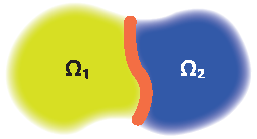
\includegraphics{chapters/chapter3/figures/blob.pdf}
\end{minipage}
\begin{minipage}{0.4\textwidth}
\begin{align*}
  E(\rOmega_{1}\cup\rOmega_2) &= E(\rOmega_1) + E(\rOmega_2) + W_{12} \qquad \\
  & \overset{?}{=}\mathcal{E}(\rOmega_1)+\mathcal{E}(\rOmega_2)
\end{align*}
\end{minipage}
\caption{
	The energy of an isolated system is the sum of the energies of its subsystems (as defined when they are isolated as well) plus the interaction among them, $W_{12}$, whose magnitude scales as the area of the interface, depicted in red. When defining the energies of individual subsystems, $\mathcal{E}$, $W_{12}$ has to be arbitrarily partitioned among them. \label{fig:energy-partition}}
\end{figure}

Let us consider a mono-atomic fluid interacting through pair potentials, $v(|\mathbf{R}_n-\mathbf{R}_m|)$, and define the atomic energies as \citep{Marcolongo2014,Ercole2016}:
\begin{equation}
  e_{\smallgamma,n}(\rGamma) =
  \frac{1}{2M_n}(\mathbf{P}_{n})^{2} + \frac{1}{2}\sum_{m\ne n}
  v(|\mathbf{R}_{n}-\mathbf{R}_{m}|)
  (1+\gamma_{nm}), \label{eq:Lambda-atomic-energies}
\end{equation}
where $\gamma_{nm}=-\gamma_{mn}$ is \emph{any} antisymmetric matrix.
As the inter-atomic potential appearing in Eq.~\eqref{eq:Lambda-atomic-energies} is symmetric with respect to the atomic indices, it is clear that the sum of all the atomic energies does not depend on $\gamma$, thus making any choice of $\gamma$ equally permissible. This trivial observation has deep consequences on the theory of thermal fluctuations and transport, because the value of the macroscopic energy flux, instead, depends explicitly on $\gamma$, thus making one fear that the resulting transport coefficients would depend on $\gamma$ as well. Using the same manipulations that lead from Eqs.~\eqref{eq:epsilon-classical} and \eqref{eq:atomic-energies} to Eq.~\eqref{eq:J-classical}, for any choice of the $\gamma$ matrix in Eq.~\eqref{eq:Lambda-atomic-energies}, a corresponding expression for the macroscopic energy flux can be found, reading \citep{Marcolongo2014,Ercole2016}:
\begin{equation}
  \mathbf{J}_{\smallgamma}^\smallE=\mathbf{J}^\smallE+
  \frac{1}{2 \rOmega}\sum_{n,m\ne n}\gamma_{nm} \Bigl ( v_{nm} \mathbf{V}_{n} + \bigl (\mathbf{V}_{n}\cdot \nabla_{\mathbf{R}_n} v_{nm} \bigr )  (\mathbf{R}_{n}-\mathbf{R}_{m}) \Bigr ), \label{eq:Lambda-classical-current}
\end{equation}
where $v_{nm}= v(|\mathbf{R}_{n} - \mathbf{R}_{m}|)$.

\begin{figure}
    \begin{center}
        \subfigure[\label{fig:argon-gauge-acf}]{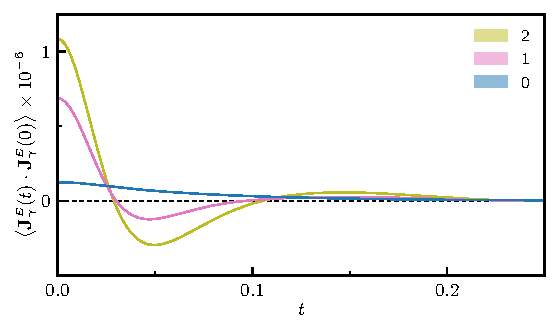
\includegraphics[width=10cm]{chapters/chapter3/figures/handbook_argon_egauge_acf.pdf}}
        \subfigure[\label{fig:argon-gauge-kappa}]{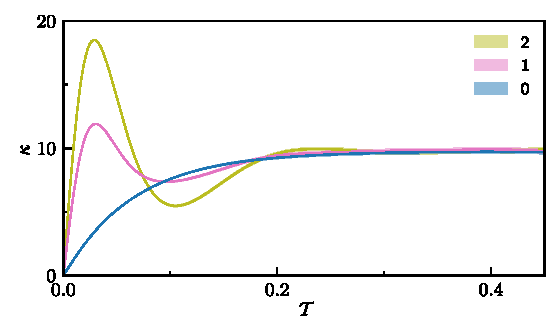
\includegraphics[width=10cm]{chapters/chapter3/figures/handbook_argon_egauge_kappa.pdf}}
    \end{center}
	\caption{(a) Time correlation functions of the modified macroscopic energy flux of a Lennard-Jones fluid, at the conditions described in the text, as defined in Eq.~\eqref{eq:Lambda-classical-current}, for different definitions of the $\gamma$ matrix. The ``0'' line refers to the standard definition ($\gamma = 0$), whereas the labels ``1'' and ``2'' correspond to two other (arbitrary) definitions of $\gamma$ as described in \cite{Ercole2016}.
    (b) Integral of the time correlation functions displayed in Fig.~\ref{fig:argon-gauge-acf}, multiplied by the prefactor appearing in the GK relation, Eq.~\eqref{eq:GK-complete}, as a function of the upper limit of integration. The barely visible shaded area surrounding each line is an indication of the error bars, as estimated by standard block analysis. Units are Lennard-Jones units ($M=\sigma=\varepsilon=1$). \label{fig:argon-gauge}}
\end{figure}

As a specific example, \cite{Ercole2016} ran MD simulations for a Lennard-Jones monoatomic fluid described by the inter-atomic potential $v(r)=\epsilon \left [ \left ( \frac{\sigma}{r}\right )^{12} - \left ( \frac{\sigma}{r}\right )^{6}\right ] $ at temperature $T=1.86 \frac{\epsilon}{k_B}$ and density $\rho=0.925 \sigma^{-3}$. In Fig.~\ref{fig:argon-gauge-acf} we display the resulting macroscopic energy-flux autocorrelation function corresponding to different choices of the $\gamma$ matrix in Eqs.~\eqref{eq:Lambda-atomic-energies} and \eqref{eq:Lambda-classical-current}. Fig.~\ref{fig:argon-gauge-acf} clearly shows that the $\langle \mathbf{J}^\smallE_{\gamma}(t) \cdot\mathbf{J}^\smallE_{\gamma}(0) \rangle$ correlation functions dramatically depend on the $\gamma$ matrices in Eqs.~\eqref{eq:Lambda-atomic-energies} and \eqref{eq:Lambda-classical-current}.  Notwithstanding, the integrals of all these time correlation functions tend to the same limit at large integration times, as shown in Fig.~\ref{fig:argon-gauge-kappa}.

In order to get insight into this remarkable invariance property, let us inspect the difference between the generalized flux in Eq.~\eqref{eq:Lambda-classical-current} and the standard expression of Eq.~\eqref{eq:J-classical}:
\begin{equation}
  \rDelta\mathbf{J}^\smallE_{\smallgamma} =\mathbf{J}^\smallE_{\smallgamma}-\mathbf{J}^\smallE  =\frac{\mathrm{d}}{\mathrm{dt}}\frac{1}{4 \rOmega} \sum_{n,m\ne n}  \gamma_{nm} \, v(|\mathbf{R}_{n}-\mathbf{R}_{m}|)  (\mathbf{R}_{n}-\mathbf{R}_{m}). \label{eq:DeltaJ}
\end{equation}
We see that the two different expressions for the macroscopic energy flux differ by a total time derivative of a bounded phase-space vector function. In the following, we show that this is a consequence of energy conservation and extensivity and a sufficient condition for the corresponding thermal conductivities to coincide.

The very possibility of defining an energy current density, from which the energy fluxes of Eq.~\eqref{eq:J-classical} and \eqref{eq:Lambda-classical-current} ultimately depend, stems from energy extensivity. The considerations illustrated in Fig.~\ref{fig:energy-partition} indicate that any two densities, $e'(\mathbf{r},t)$ and $e(\mathbf{r},t)$, whose integrals over a macroscopic volume differ by a quantity that scales as the volume boundary, should be considered as equivalent. This equivalence can be expressed by the condition that two equivalent densities differ by the divergence of a (bounded) vector field:
\begin{equation}
  e'(\mathbf{r},t)=e(\mathbf{r},t) - \nabla\cdot \bm{p}(\mathbf{r},t). \label{eq:gauge_transformation}
\end{equation}
In a sense, two equivalent energy densities can be thought of as different \emph{gauges} of the same scalar field. Energy is also conserved: because of this, for any given gauge of the energy density, $e(\mathbf{r},t)$, an energy current density can be defined, $\bm{j}(\mathbf{r},t)$, so as to satisfy the continuity equation, Eq.~\eqref{eq:continuity}. By combining Eqs.~\eqref{eq:gauge_transformation} and \eqref{eq:continuity} we see that energy current densities and macroscopic fluxes transform under a gauge transformation as:
\begin{align}
 \bm{j}'(\mathbf{r},t) & = \bm{j}(\mathbf{r},t) + \dot{\bm{p}}(\mathbf{r},t), \label{eq:current_density_gauge} \\
  \mathbf{J}'(t) & = \mathbf{J}(t) + \dot{\mathbf{P}}(t), \label{eq:macroscopic_flux_gauge}
\end{align}
where $\mathbf{P}(t)=\frac{1}{\rOmega} \int\bm{p}(\mathbf{r},t)d\mathbf{r}$. We
conclude that the macroscopic energy fluxes in two different energy gauges differ by the total time derivative of a bounded phase-space vector function.

We now show that the energy fluxes of the same system in two different energy gauges, $e$ and $e'$, differing by a bounded total time derivative, as in Eq.~\eqref{eq:macroscopic_flux_gauge}, result in the same heat conductivity, as given by the Green-Kubo formula, Eq.~\eqref{eq:GK-complete}. More generally, the Onsager coefficients coupling two fluxes, $\mathbf{J}^1$ and $\mathbf{J}^2$, do not depend on the gauge of either one of them. In fact, let $\left(\mathbf{J}^1\right)' = \mathbf{J}^1 + \dot{\mathbf{P}}$; one has:
\begin{equation}
  \begin{aligned}
    \left (L^{11} \right)' &= \frac{\rOmega}{2 k_B }\int_{-\infty}^{+\infty} \left \langle \left (\mathbf{J}_1(t)+\dot{\mathbf{P}}(t) \right ) \cdot  \left (\mathbf{J}_1(0)+\dot{\mathbf{P}}(0)\right ) \right \rangle dt \\
    &= L^{11} + \frac{\rOmega}{2 k_B } \left[ \left .  \left \langle \mathbf{P}(t) \cdot \dot{\mathbf{P}}(0) \right \rangle \right |^{+\infty}_{-\infty} + \left .  2 \Bigl \langle \mathbf{P}(t) \cdot \mathbf{J}_1(0) \Bigr \rangle \right |^{+\infty}_{-\infty} \right] .
  \end{aligned} \label{eq:L=L'}
\end{equation}

The expectation of the time-lagged products in Eq.~\eqref{eq:L=L'} is equal to the products of two expectations at large time lag. As the equilibrium expectations of both a total time derivative and a current vanish, we conclude that $\left (L^{11}\right )'=L^{11}$. A slight generalization of this argument, also using microscopic reversibility as in \cite{Onsager1931a,Onsager1931b}, allows us to conclude that $\left (L^{12} \right )'=L^{12}$ and that, in general, $\kappa'=\kappa$.


\section{Molecular fluids} \label{sec:MolecularFluids}
In a one-component molecular fluid such as liquid water or, say, ethanol, there are in general $Q$ fluxes interacting with each other through Onsagers' Eq.~\eqref{eq:onsager}, where $Q$ is the number of atomic species in a molecule. The requirement that atoms are bound in molecules of fixed composition, however, sets a number of constraints that substantially simplify the treatment of heat transport, making the molecular case similar to the one-component one.

Let us consider a molecule of chemical formula $A_{N_A} B_{N_B}\cdots$, where $A, B,\cdots$ indicate atomic species, and $N_A,N_B,\cdots$ the corresponding atomic stoichiometric indices. For each atomic species we define the normalized number flux as:
\begin{equation}
  \mathbf{J}^X = \frac{1}{N_X}\sum_{n\in X} \mathbf{V}_n. \label{eq:JX}
\end{equation}
If we indicate by $M_X$ the atomic mass of species $X$, momentum conservation requires that $\sum_X M_X N_X \mathbf{J}^X = 0$ in the center-of-mass reference frame. The flux $\mathbf{J}^{XY} = \mathbf{J}^{X}-\mathbf{J}^{Y}$ is the total time derivative of a bounded vector, because its integral is the sum over all the molecules of the difference between the average atomic positions of either species within a same molecule, which is obviously bounded if molecules do not dissociate. As any number flux $\mathbf{J}^X$ can be expressed as a linear combination of the total momentum and of several $\mathbf{J}^{XY}$ fluxes, each of them is the total time derivative of a bounded vector. Therefore, the Onsager coefficient coupling any of these atomic fluxes with any other, or with the energy flux, vanishes. We conclude that energy is the only conserved quantity relevant for heat transport in a molecular fluid, and that the energy-flux autocorrelation function directly yields the thermal conductivity, as in Eq.~\eqref{eq:GK}.

  % Gauge invariance

%\chapterauthor{Author Name}{Author Affiliation}
\chapterauthor{Second Author}{Second Author Affiliation}
\chapter{Basic Concepts}

A component part for an electronic item is
manufactured at one of three different factories, and then delivered to
the main assembly line.Of the total number supplied, factory A supplies
50\%, factory B 30\%, and factory C 20\%. Of the components
manufactured at factory A, 1\% are faulty and the corresponding
proportions for factories B and C are 4\% and 2\% respectively. A
component is picked at random from the assembly line. What is the
probability that it is faulty?

\section{Introduction}\label{intro}
The term reliability usually refers to the probability that a
component or system will operate satisfactorily either at any particular
instant at which it is required or for a certain length of
time. Fundamental to quantifying reliability s a knowledge of how to
define, assess and combine probabilities \cite{Bontempi2005Adaptive}. This may hinge on identifying the
form of the variability which is nherent n most processes. If all
components had a fixed known lifetime there would be no need to model
reliability.

\begin{enumerate}[1.]
\item A component part for an electronic item is
manufactured at one of three different factories.

\item A component part $x$ for an electronic item is
manufactured at one of three different factories.
\begin{enumerate}
\item A component part for an electronic item is
manufactured at one of three different factories.

\item A component part $x$ for an electronic item is
manufactured at one of three different factories.
\begin{enumerate}[iv.]
\item A component part for an electronic item is
manufactured at one of three different factories.

\item A component part $x$ for an electronic item is
manufactured at one of three different factories.

\item A component part for an electronic item is
manufactured at one of three different factories.

\item A component part 1, 2, 3, 4 for an electronic item is
manufactured at one of three different factories.

\item A component part for enumerate list of an electronic item is
manufactured at one of three different factories.

\end{enumerate}

\item A component part for an electronic item is
manufactured at one of three different factories.

\item A component part 1, 2, 3, 4 for an electronic item is
manufactured at one of three different factories.

\item A component part for enumerate list of an electronic item is
manufactured at one of three different factories.

\end{enumerate}

\item A component part for an electronic item is
manufactured at one of three different factories.

\item A component part 1, 2, 3, 4 for an electronic item is
manufactured at one of three different factories.

\item A component part for enumerate list of an electronic item is
manufactured at one of three different factories.

\end{enumerate}

\subsection{A component part}
A component part for an electronic item is
manufactured at one of three different factories, and then delivered to
the main assembly line.Of the total number supplied, factory A supplies
50\%, factory B 30\%, and factory C 20\%. Of the components
manufactured at factory A, 1\% are faulty and the corresponding
proportions for factories B and C are 4\% and 2\% respectively. A
component is picked at random from the assembly line. What is the
probability that it is faulty \cite{ilyas2004hsn}?
A component part for an electronic item is
manufactured at one of three different factories, and then delivered to
the main assembly line. Of the total number supplied, factory A supplies
50\%, factory B 30\%, and factory C 20\%. Of the components
manufactured at factory A, 1\% are faulty and the corresponding
proportions for factories B and C are 4\% and 2\% respectively. A
component is picked at random from the assembly line. What is the
probability that it is faulty?
A component part for an electronic item is
manufactured at one of three different factories, and then delivered to
the main assembly line.Of the total number supplied, factory A supplies
50\%, factory B 30\%, and factory C 20\%. Of the components
manufactured at factory A, 1\% are faulty and the corresponding
proportions for factories B and C are 4\% and 2\% respectively. A
component is picked at random from the assembly line. What is the
probability that it is faulty?

\begin{VF}
``A Process is a structured, measured set of activities designed to produce a specific output for a particular customer
or market---A process is thus a specific ordering of work activities across time and space, with a beginning, an end.
and clearly defined inputs and outputs: a structure for action.''

\VA{Thomas Davenport}{Senior Adjutant to the Junior Marketing VP}
\end{VF}


\begin{table}%1
%\noautomaticrules
\tabletitle{Now we are engaged $(a_g^a)$ $\big(a_g^a\big)$ in a great civil war, testing whether that
nation, or any nation so conceived.}%
\begin{tabular}{lccc}
\tch{Scene}    &\tch{Reg. fts.} &\tch{Hor. fts.} &\tch{Ver. fts.}\\
Ball &19, 221 &4, 598   &3, 200\\
Pepsi$^a$&46, 281 &6, 898 &5, 400\\
Keybrd$^b$   &27, 290 &2, 968 &3, 405\\
Pepsi    &14, 796 &9, 188 &3, 209\\
\end{tabular}
\end{table}

\textbf{MultiRelational $k$-Anonymity.} Most works on $k$-anonymity focus on anonymizing a single data table; however, a real-life \cite{diamantaras1996pcn} database usually contains multiple relational tables. This has proposed a privacy model called \emph{MultiR $k$-anonymity} to ensure $k$-anonymity on multiple relational tables. Their model assumes that a relational database contains a person-specific table $PT$ and a set of tables $T_1,\cdots,T_n$, where $PT$ contains a person identifier $Pid$ and some sensitive attributes, and $T_i$, for $1 \leq i \leq n$, contains some foreign keys, some attributes in $QID$, and sensitive attributes. The general privacy notion is to ensure that for each record owner $o$ contained in the join of all tables $PT \Join T_1 \Join \cdots \Join T_n$, there exists at least $k-1$ other record owners share the same $QID$ with $o$. It is important to emphasize that the $k$-anonymization is applied at the \emph{record owner} level, not at the \emph{record} level in traditional $k$-anonymity. This idea is similar to $(X,Y)$-anonymity, where $X=QID$ and $Y=\{Pid\}$.

Most works on $k$-anonymity focus on anonymizing a single data table; however, a real-life \cite{diamantaras1996pcn} database usually contains multiple relational tables. This has proposed a privacy model called \emph{MultiR $k$-anonymity} to ensure $k$-anonymity on multiple relational tables. Their model assumes that a relational database contains a person-specific table $PT$ and a set of tables $T_1,\cdots,T_n$, where $PT$ contains a person identifier $Pid$ and some sensitive attributes, and $T_i$, for $1 \leq i \leq n$, contains some foreign keys, some attributes in $QID$, and sensitive attributes. The general privacy notion is to ensure that for each record owner $o$ contained in the join of all tables $PT \Join T_1 \Join \cdots \Join T_n$, there exists at least $k-1$ other record owners share the same $QID$ with $o$. It is important to emphasize that the $k$-anonymization is applied at the \emph{record owner} level, not at the \emph{record} level in traditional $k$-anonymity. This idea is similar to $(X,Y)$-anonymity, where $X=QID$ and $Y=\{Pid\}$.

\begin{table}[b!]%2
\tabletitle[Short Table Caption]{Now we are engaged $(a_g^a)$ $\big(a_g^a\big)$ in a great civil war, testing whether that
nation, or any nation so conceived.}%}{%
\begin{tabular}{lccc}
\tch{Scene}    &\tch{Reg. fts.} &\tch{Hor. fts.} &\tch{Ver. fts.}\\
\multicolumn{4}{@{}l@{}}{\tsh{Table Head}}\\[3pt]\hline\\[-6pt]
Ball &19, 221 &4, 598   &3, 200\\
Pepsi &46, 281 &6, 898 &5, 400\\
Keybrd   &27, 290 &2, 968 &3, 405\\
Pepsi    &14, 796 &9, 188 &3, 209\\
\end{tabular}
\end{table}

% \begin{shadebox} %This doesn’t work with the pdftex engine -- see the manual.
% A component part for an electronic item is
% manufactured at one of three different factories, and then delivered to
% the main assembly line.Of the total number supplied, factory A supplies
% 50\%, factory B 30\%, and factory C 20\%. Of the components
% manufactured at factory A, 1\% are faulty and the corresponding
% proportions for factories B and C are 4\% and 2\% respectively. A
% component is picked at random from the assembly line. What is the
% probability that it is faulty?
% \end{shadebox}

In most literature on PPDP, they \cite{jolliffe2002pca} consider a more relaxed, yet more practical, notion of privacy protection by assuming limited attacker's background knowledge. Below, the term ``victim" refers to the record owner being linked. We can broadly classify linking models to two families.

\begin{extract}
A component part for an electronic item is \cite{hyvarinen2001ica}
manufactured at one of three different factories, and then delivered to
the main assembly line.Of the total number supplied, factory A supplies
50\%, factory B 30\%, and factory C 20\%. Of the components
manufactured at factory A, 1\% are faulty and the corresponding
proportions for factories B and C are 4\% and 2\% respectively.
\end{extract}


One family considers a privacy threat occurs when an attacker is able to link a record owner to a record in a published data table, to a sensitive attribute in a published data table, or to the published data table itself. We call them \emph{record linkage}, \emph{attribute linkage}, and \emph{table linkage}, respectively. In all types of linkages, we assume that the attacker knows the $QID$ of the victim. In record and attribute linkages, we further assume that the attacker knows the presence of the victim's record in the released table, and seeks to identify the victim's record and/or sensitive information from the table \cite{yao2002can}. In table linkage, the attack seeks to determine the present or absent of the victim's record in the released table. A data table is considered to privacy preserved if the table can effectively prevent the attacker from successfully performing these types of linkages on the table \cite{madden2002tta}. Sections~\ref{intro}-\ref{sec:reclinkage} study this family of privacy models.
\begin{equation}
\mbox{var}\widehat{\Delta} = \sum_{j = 1}^t \sum_{k = j+1}^t
\mbox{var}\,(\hat{\alpha}_j - \hat{\alpha}_k)  = \sum_{j = 1}^t
\sum_{k = j+1}^t \sigma^2(1/n_j + 1/n_k). \label{2delvart2}
\end{equation}


An obvious measure of imbalance is just the difference in the
number of times the two treatments are allocated
\begin{equation}
D_n = \mathcal{M}|n_A - n_B|. \label{2deffD}
\end{equation}
For rules such as deterministic allocation, for which the expected
value of this difference can be calculated, we obtain the population
value ${\cal D}_n$.

\begin{shortbox}
\Boxhead{Box Title Here}
Another family aims at achieving the \emph{uninformative principle}: The published table should provide the attacker with little additional information beyond the background knowledge. There should not be a large difference between the prior and posterior beliefs; otherwise, there is a privacy threat~\cite{jain2004ass, jolliffe2002pca}. Many privacy models in this family are designed for statistical database and do not distinguish attributes in $T$ into $QID$, but some of them could also thwart record, attribute, and table linkages. Section~\ref{intro} studies this family of privacy models.

Let $m$ be a prime number. With the addition and multiplication as
defined above, $Z_m$ is a field.
\end{shortbox}

\begin{theorem}\label{1th:Z_m}
Let $m$ be a prime number. With the addition and multiplication as
defined above, $Z_m$ is a field.
\end{theorem}

\begin{proof}
Most of the proof of this theorem is routine.  It is clear that $0\in Z_m$
and $1\in Z_m$ are the
zero element and identity element. If $a\in Z_m$ and $a\ne 0$, then $m-a$
is the additive inverse of $a$. If $a\in Z_m$ and $a\ne 0$, then the
greatest common divisor of $a$ and $m$ is 1, and hence
there exist integers $s$ and $t$ such that $sa+tm=1$. Thus $sa=1 -tm$ is
congruent to 1 modulo $m$. Let $s^*$ be the integer in $Z_m$
congruent to $s$
modulo $m$. Then we also have $s^*a\equiv 1\  \mbox{mod}\ m$. Hence $s^*$
is
the multiplicative inverse of $a$ modulo $m$. Verification of the rest of
the field properties is now routine.\end{proof}



\section{Record Linkage Model}\label{sec:reclinkage}

In the privacy attack of \emph{record linkage}, some value $qid$ on $QID$ identifies a small number of records in the released table $T$,
called a \emph{group}. If the victim's $QID$ matches the value
$qid$, the victim is vulnerable to being linked to the small
number of records in the group \cite{madden2005taq}. In this case, the attacker faces
only a small number of possibilities for the victim's record, and
with the help of additional knowledge, there is a chance that the
attacker could uniquely identify the victim's record from the
group.


%%%\begin{table}
%%%    \tabletitle{Examples for illustrating attacks}
%%%    \begin{tabular}{|c|c|c|c|}
%%%        \hline
%%%        \textbf{Job} & \textbf{Sex} & \textbf{Age} & \textbf{Disease} \\
%%%        \hline
%%%        Engineer & Male & 35 & Hepatitis \\
%%%        Engineer & Male & 38 & Hepatitis \\
%%%        Lawyer & Male & 38 & HIV \\
%%%        Writer & Female & 30 & Flu \\
%%%        Writer & Female & 30 & HIV \\
%%%        Dancer & Female & 30 & HIV \\
%%%        Dancer & Female & 30 & HIV \\
%%%        \hline
%%%    \end{tabular}
%%%    \label{table:rawpatient}
%%%\end{table}



\subsection{A component part}
A component part for an electronic item is
manufactured at one of three different factories, and then delivered to
the main assembly line.Of the total number supplied, factory A supplies
50\%, factory B 30\%, and factory C 20\%. Of the components
manufactured at factory A, 1\% are faulty and the corresponding
proportions for factories B and C are 4\% and 2\% respectively. A
component is picked at random from the assembly line. What is the
probability that it is faulty?



\begin{figure}

\includegraphics[width=350pt, height=200pt]{chapters/chapterex/figures/cat.eps}
%%\centerline{\epsfig{/chapters/chapterex/figures/cat.eps,width=.8\textheight,height=.4\textwidth}}
\caption[List of figure caption goes here]{Figure caption goes here.}
\end{figure}



\begin{figure}[htb]

\includegraphics[width=200pt, height=200pt]{chapters/chapterex/figures/cat}
%%\centerline{\epsfig{figure=cat.eps,width=.5\textheight,height=.4\textwidth}}
\caption[Short figure caption]{Figure caption goes here. Figure caption goes here.
Figure caption goes here. Figure caption goes here. Figure caption goes here.
Figure caption goes here.}
\end{figure}





\begin{figure}
\begin{center}
\subfigure[\label{f8a}]{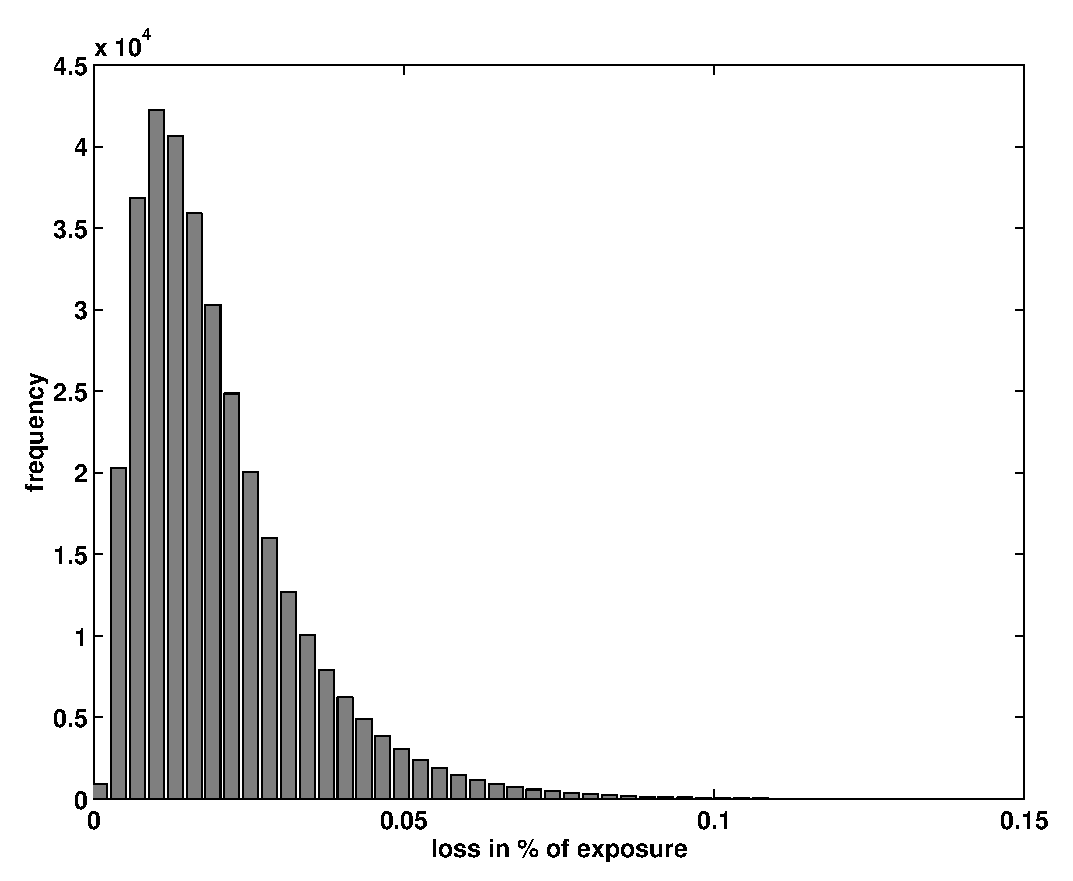
\includegraphics[angle=90,width=7cm,height=7cm,angle=-90]{chapters/chapterex/figures/Histogram.eps}}
\subfigure[\label{f8b}]{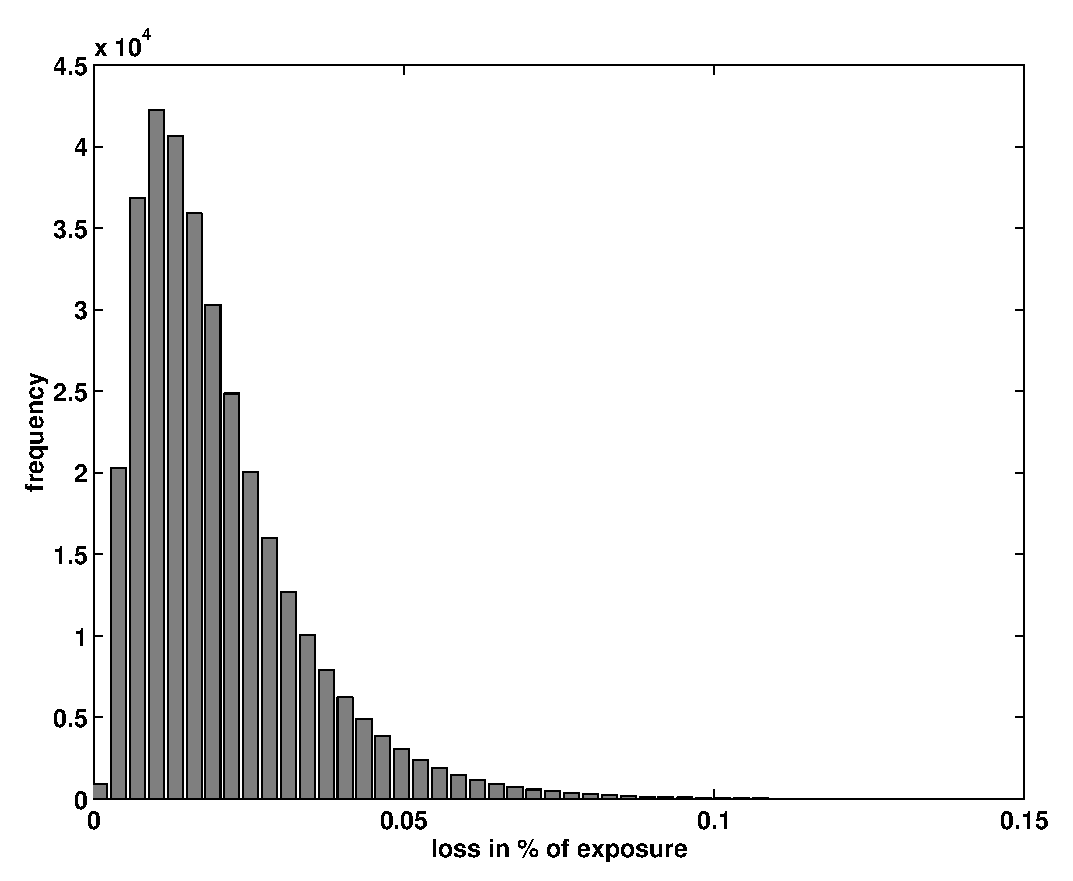
\includegraphics[angle=90,width=7cm,height=7cm,angle=-90]{chapters/chapterex/figures/Histogram.eps}}
\end{center}
\caption[The bar charts depict the different risk contributions]{The bar charts depict the different risk contributions (top: 99\% quantile, bottom: 99.9\% quantile) of the business areas of a bank. The black bars
are based on a Var/Covar approach, the white ones correspond to shortfall risk.}
\end{figure}

\subsubsection{H3 A component part }
A component part for an electronic item is
manufactured at one of three \cite{mardia1979ma} different factories, and then delivered to
the main assembly line.Of the total number supplied, factory A supplies
50\%, factory B 30\%, and factory C 20\%. Of the components
manufactured at factory A, 1\% are faulty and the corresponding
proportions for factories B and C are 4\% and 2\% respectively. A
component is picked at random from the assembly line. What is the
probability that it is faulty?


A fundamental notion \cite{yao2002can} is that of a\index{subspace}\index{vector
space!subspace of} subspace of $F^n$. Let $V$ be a nonempty subset of
$F^n$. Then $V$ is a {\it subspace} of $F^n$ provided $V$ is closed
under vector addition and scalar multiplication, that is,
\begin{enumerate}
\item[\rm (a)] For all $u$ and $v$ in $V$, $u+v$ is
also in $V$.
\item[\rm (b)] For all $u$ in $V$ and $c$ in $F$, $cu$ is
in $V$.
\end{enumerate}
Let $u$ be in the subspace $V$. Because $0u=0$,
it follows that the zero vector is in $V$. Similarly, $-u$ is in $V$
for all $u$ in $V$. A simple example of a subspace of $F^n$ is the set
of all vectors $(0,a_2,\ldots,a_n)$ with first coordinate equal to 0.
The zero vector itself is a subspace.

\begin{definition}\label{1def:linearcomb}{\rm
Let $u^{(1)},u^{(2)},\ldots,u^{(m)}$ be vectors in $F^n$, and let
$c_1,c_2,\ldots,c_m$ be scalars. Then the vector
\[c_1u^{(1)}+c_2u^{(2)}+\cdots+c_mu^{(m)}\]
is called a {\it linear combination} \index{linear combination} of $u^{(1)},u^{(2)},\ldots,u^{(m)}$.
If $V$ is a subspace of $F^n$, then $V$ is closed under vector addition and
scalar multiplication, and it follows easily by induction that a
linear combination of vectors in $V$ is also a vector in $V$. Thus
{\it subspaces
are closed under linear combinations}; in fact, this can be taken as the
defining property of subspaces.
The vectors $u^{(1)},u^{(2)},\ldots,u^{(m)}$ {\it span} $V$ \index{spanning set}
(equivalently, form a {\it spanning set} of $V$) provided every vector in
$V$
is a linear combination of $u^{(1)},u^{(2)},\ldots,u^{(m)}$. The zero
vector can be written as a linear combination of
$u^{(1)},u^{(2)},\ldots,u^{(m)}$ with all scalars equal to 0; this is a
{\it trivial linear combination}.\index{linear combination!trivial} The vectors
$u^{(1)},u^{(2)},\ldots,u^{(m)}$ are {\it linearly dependent} provided
there are scalars $c_1,c_2,\ldots,c_m$, not all of which are zero, such
that
\[c_1u^{(1)}+c_2u^{(2)}+\cdots+c_mu^{(m)}=0,\]
that is, the zero vector can be written as a {\it nontrivial linear \index{linear combination!nontrivial}
combination} of $u^{(1)},u^{(2)},\ldots,u^{(m)}$.
For example, the vectors $(1,4), (3,-1)$, and $(3,5)$ in $\Re^2$ are
linearly
dependent since
\[3(1,4)+1(3,-2)-2(3,5)=(0,0).\] Vectors are {\it linearly independent} provided  they are not linearly dependent.\index{linearly independent}
The vectors
$u^{(1)},u^{(2)},\ldots,u^{(m)}$ are a {\it basis} \index{basis} of $V$ provided they are
linearly independent and span $V$.
By an {\it ordered basis} \index{basis!ordered} we mean a basis in which the vectors of the basis are listed
in a specified order; to indicate that we have an ordered basis we write
$(u^{(1)},u^{(2)},\ldots,u^{(m)})$.
A spanning set $S$ of $V$ is a \index{spanning set!minimal} {\it minimal spanning set of $V$} provided that
each set
of vectors obtained from $S$ by removing a vector is not a spanning set
for $V$.
A linearly independent set $S$ of vectors of $V$ is a {\it maximal linearly \index{linearly independent!maximal}
independent set of vectors of $V$} provided that for each vector $w$ of
$V$ that
is not in $S$, $S\cup\{w\}$ is  linearly dependent (when this happens,
$w$ must be  a linear combination of the vectors in
$S$).\hfill{$\Box$}
}\end{definition}

In addition to matrix addition, subtraction, and multiplication, there is
one additional operation that we define now. It's perhaps the simplest of
them all. Let $A=[a_{ij}]$ be an $m$ by $n$ matrix and let $c$ be a
number \cite{hyvarinen2001ica}. Then the matrix $c\cdot A$, or simply $cA$, is the $m$ by $n$
matrix obtained by multiplying each entry of $A$ by $c$:
\[c A=[ca_{ij}].\]\index{matrix!scalar multiplication} \index{matrix!scalar multiple of}
The matrix $c A$ is called a {\it scalar multiple} of $A$.

\begin{VT1}

\VH{Think About It...}

Commonly thought of as the first modern computer, ENTAC was built in 1944. It took up more space than an 18-wheeler's
tractor trailer and weighed more than 17 Chevrolet Camaros. It consumed 140,000 watts of electricity while executing
up to 5,000 basic arithmetic operations per second. One of today's popular microprocessors, the 486, is built on a
tiny piece of silicon about the size of a dime.

\VT
With the continual expansion of capabilities, computing power will eventually exceed the capacity for human
comprehension or human control.

\VTA{The Information Revolution}{Business Week}
\end{VT1}


\section{Glossary}
\begin{Glossary}
\item[360 Degree Review] Performance review that includes feedback from superiors, peers, subordinates, and clients.
\item[Abnormal Variation] Changes in process performance that cannot be accounted for by typical day-to-day variation. Also referred to as
non-random variation.
\item[Acceptable Quality Level (AQL)] The minimum number of parts that must comply with quality standards, usually stated as a percentage.
\item[Activity] The tasks performed to change inputs into outputs.
\item[Adaptable] An adaptable process is designed to maintain effectiveness and efficiency as requirements change. The process is
deemed adaptable when there is agreement among suppliers, owners, and customers that the process will meet
requirements throughout the strategic period.
\end{Glossary}






%\part{Climate Risks in Public Health and Epidemiology}



\bibliographystyle{plainnat}
%\bibliography{bibtex_example}
\bibliography{bibliography}

\printindex

\end{document}